\documentclass[
ngerman,
toc=listof,
toc=bibliography,
footnotes=multiple,
parskip=half,
numbers=noendperiod
]{scrartcl}
\pdfminorversion=5
\usepackage[utf8]{inputenc}

% !TEX root = document.tex

\newcommand{\titel}{Titel}
\newcommand{\untertitel}{Untertitel}
\newcommand{\kompletterTitel}{\titel{} -- \untertitel}

\newcommand{\autorName}{Matthias Fischer}
\newcommand{\autorGeburt}{21.12.1994 in Dinklage}
\newcommand{\autorAnschrift}{Gartenstr. 29}
\newcommand{\autorOrt}{49635 Badbergen}
\newcommand{\autorMatrikel}{700643}
\newcommand{\autorStudiengruppe}{15DWF1}

\newcommand{\betreuer}{Herr iwas.}
\newcommand{\zweitBetreuer}{Herr sowieso}
\newcommand{\modul}{Grundlagen von iwas}

\newcommand{\betriebLogo}{hs-logo.png}
\newcommand{\betriebName}{xxxx}
\newcommand{\betriebAnschrift}{xxxxx}
\newcommand{\betriebOrt}{xxxxx xxx}

\newcommand{\betreff}{Praxis-Transfer-Projekt}
\newcommand{\studiengang}{Wirtschaftsinformatik}
\newcommand{\abgabeTermin}{17.05.2017}

% !TEX root = document.tex

% Anpassung an Landessprache ---------------------------------------------------
\usepackage{babel}

% Umlaute ----------------------------------------------------------------------
%   Umlaute/Sonderzeichen wie äüöß direkt im Quelltext verwenden (CodePage).
%   Erlaubt automatische Trennung von Worten mit Umlauten.
% ------------------------------------------------------------------------------
\usepackage[T1]{fontenc}
\usepackage{textcomp} % Euro-Zeichen etc.

% Schrift ----------------------------------------------------------------------
\usepackage{lmodern} % bessere Fonts
\usepackage{relsize} % Schriftgröße relativ festlegen

% Dummy Texte ------------------------------------------------------------------
\usepackage{blindtext}

% Tabellen ---------------------------------------------------------------------
\PassOptionsToPackage{table}{xcolor}
\usepackage{tabularx}

% für lange Tabellen
\usepackage{longtable}
\usepackage{array}
\usepackage{ragged2e}
\usepackage{lscape}
\newcolumntype{w}[1]{>{\raggedleft\hspace{0pt}}p{#1}} % Spaltendefinition rechtsbündig mit definierter Breite

% Grafiken ---------------------------------------------------------------------
\usepackage[dvips,final]{graphicx} % Einbinden von JPG-Grafiken ermöglichen
\usepackage{graphics} % keepaspectratio
\usepackage{floatflt} % zum Umfließen von Bildern
\graphicspath{{images/}} % hier liegen die Bilder des Dokuments

% Sonstiges --------------------------------------------------------------------
\usepackage[titles]{tocloft} % Inhaltsverzeichnis DIN 5008 gerecht einrücken
\usepackage{amsmath,amsfonts} % Befehle aus AMSTeX für mathematische Symbole
\usepackage{enumitem} % anpassbare Enumerates/Itemizes
\usepackage{xspace} % sorgt dafür, dass Leerzeichen hinter parameterlosen Makros nicht als Makroendezeichen interpretiert werden

\usepackage{makeidx} % für Index-Ausgabe mit \printindex
\usepackage[printonlyused]{acronym} % es werden nur benutzte Definitionen aufgelistet

% Einfache Definition der Zeilenabstände und Seitenränder etc.
\usepackage{setspace}
\usepackage{geometry}

% Symbolverzeichnis
\usepackage[intoc]{nomencl}
\let\abbrev\nomenclature
\renewcommand{\nomname}{Abkürzungsverzeichnis}
\setlength{\nomlabelwidth}{.25\hsize}
\renewcommand{\nomlabel}[1]{#1 \dotfill}
\setlength{\nomitemsep}{-\parsep}

\usepackage{varioref} % Elegantere Verweise. „auf der nächsten Seite“
\usepackage{url} % URL verlinken, lange URLs umbrechen etc.

\usepackage{chngcntr} % fortlaufendes Durchnummerieren der Fußnoten
% \usepackage[perpage]{footmisc} % Alternative: Nummerierung der Fußnoten auf jeder Seite neu

\usepackage{ifthen} % bei der Definition eigener Befehle benötigt
\usepackage{todonotes} % definiert u.a. die Befehle \todo und \listoftodos
\usepackage[square]{natbib} % wichtig für korrekte Zitierweise

% PDF-Optionen -----------------------------------------------------------------
\usepackage{pdfpages}
\pdfminorversion=5 % erlaubt das Einfügen von pdf-Dateien bis Version 1.7, ohne eine Fehlermeldung zu werfen (keine Garantie für fehlerfreies Einbetten!)
\usepackage[
    bookmarks,
    bookmarksnumbered,
    bookmarksopen=true,
    bookmarksopenlevel=1,
    colorlinks=true,
% diese Farbdefinitionen zeichnen Links im PDF farblich aus
    linkcolor=AOBlau, % einfache interne Verknüpfungen
    anchorcolor=AOBlau,% Ankertext
    citecolor=AOBlau, % Verweise auf Literaturverzeichniseinträge im Text
    filecolor=AOBlau, % Verknüpfungen, die lokale Dateien öffnen
    menucolor=AOBlau, % Acrobat-Menüpunkte
    urlcolor=AOBlau,
% diese Farbdefinitionen sollten für den Druck verwendet werden (alles schwarz)
    %linkcolor=black, % einfache interne Verknüpfungen
    %anchorcolor=black, % Ankertext
    %citecolor=black, % Verweise auf Literaturverzeichniseinträge im Text
    %filecolor=black, % Verknüpfungen, die lokale Dateien öffnen
    %menucolor=black, % Acrobat-Menüpunkte
    %urlcolor=black,
%
    %backref, % Quellen werden zurück auf ihre Zitate verlinkt
    pdftex,
    plainpages=false, % zur korrekten Erstellung der Bookmarks
    pdfpagelabels=true, % zur korrekten Erstellung der Bookmarks
    hypertexnames=false, % zur korrekten Erstellung der Bookmarks
    linktocpage % Seitenzahlen anstatt Text im Inhaltsverzeichnis verlinken
]{hyperref}

% Befehle, die Umlaute ausgeben, führen zu Fehlern, wenn sie hyperref als Optionen übergeben werden
\hypersetup{
    pdftitle={\titel -- \untertitel},
    pdfauthor={\autorName},
    pdfcreator={\autorName},
    pdfsubject={\titel -- \untertitel},
    pdfkeywords={\titel -- \untertitel},
}


% zum Einbinden von Programmcode -----------------------------------------------
\usepackage{listings}
\usepackage{xcolor}
\definecolor{hellgelb}{rgb}{1,1,0.9}
\definecolor{colKeys}{rgb}{0,0,1}
\definecolor{colIdentifier}{rgb}{0,0,0}
\definecolor{colComments}{rgb}{0,0.5,0}
\definecolor{colString}{rgb}{1,0,0}
\lstset{
    float=hbp,
	basicstyle=\footnotesize,
    identifierstyle=\color{colIdentifier},
    keywordstyle=\color{colKeys},
    stringstyle=\color{colString},
    commentstyle=\color{colComments},
    backgroundcolor=\color{hellgelb},
    columns=flexible,
    tabsize=2,
    frame=single,
    extendedchars=true,
    showspaces=false,
    showstringspaces=false,
    numbers=left,
    numberstyle=\tiny,
    breaklines=true,
    breakautoindent=true,
	captionpos=b,
}

\lstdefinelanguage{CSS}{
	morekeywords={accelerator,azimuth,background,background-attachment,
		background-color,background-image,background-position,
		background-position-x,background-position-y,background-repeat,
		behavior,border,border-bottom,border-bottom-color,
		border-bottom-style,border-bottom-width,border-collapse,
		border-color,border-left,border-left-color,border-left-style,
		border-left-width,border-right,border-right-color,
		border-right-style,border-right-width,border-spacing,
		border-style,border-top,border-top-color,border-top-style,
		border-top-width,border-width,bottom,caption-side,clear,
		clip,color,content,counter-increment,counter-reset,cue,
		cue-after,cue-before,cursor,direction,display,elevation,
		empty-cells,filter,float,font,font-family,font-size,
		font-size-adjust,font-stretch,font-style,font-variant,
		font-weight,height,ime-mode,include-source,
		layer-background-color,layer-background-image,layout-flow,
		layout-grid,layout-grid-char,layout-grid-char-spacing,
		layout-grid-line,layout-grid-mode,layout-grid-type,left,
		letter-spacing,line-break,line-height,list-style,
		list-style-image,list-style-position,list-style-type,margin,
		margin-bottom,margin-left,margin-right,margin-top,
		marker-offset,marks,max-height,max-width,min-height,
		min-width,-moz-binding,-moz-border-radius,
		-moz-border-radius-topleft,-moz-border-radius-topright,
		-moz-border-radius-bottomright,-moz-border-radius-bottomleft,
		-moz-border-top-colors,-moz-border-right-colors,
		-moz-border-bottom-colors,-moz-border-left-colors,-moz-opacity,
		-moz-outline,-moz-outline-color,-moz-outline-style,
		-moz-outline-width,-moz-user-focus,-moz-user-input,
		-moz-user-modify,-moz-user-select,orphans,outline,
		outline-color,outline-style,outline-width,overflow,
		overflow-X,overflow-Y,padding,padding-bottom,padding-left,
		padding-right,padding-top,page,page-break-after,
		page-break-before,page-break-inside,pause,pause-after,
		pause-before,pitch,pitch-range,play-during,quotes,
		-replace,richness,right,ruby-align,ruby-overhang,
		ruby-position,-set-link-source,size,speak,speak-header,
		speak-numeral,speak-punctuation,speech-rate,stress,
		scrollbar-arrow-color,scrollbar-base-color,
		scrollbar-dark-shadow-color,scrollbar-face-color,
		scrollbar-highlight-color,scrollbar-shadow-color,
		scrollbar-3d-light-color,scrollbar-track-color,table-layout,
		text-align,text-align-last,text-decoration,text-indent,
		text-justify,text-overflow,text-shadow,text-transform,
		text-autospace,text-kashida-space,text-underline-position,top,
		unicode-bidi,-use-link-source,vertical-align,visibility,
		voice-family,volume,white-space,widows,width,word-break,
		word-spacing,word-wrap,writing-mode,z-index,zoom},
	morestring=[s]{:}{;},
	sensitive,
	morecomment=[s]{/*}{*/}
}

\lstdefinelanguage{HTML5}{
	language=html,
	sensitive=true,	
	alsoletter={<>=-},	
	morecomment=[s]{<!-}{-->},
	tag=[s],
	otherkeywords={
		% General
		>,
		% Standard tags
		<!DOCTYPE,
		</html, <html, <head, <title, </title, <style, </style, <link, </head, <meta, />,
		% body
		</body, <body,
		% Divs
		</div, <div, </div>, 
		% Paragraphs
		</p, <p, </p>,
		% scripts
		</script, <script,
		% More tags...
		<canvas, /canvas>, <svg, <rect, <animateTransform, </rect>, </svg>, <video, <source, <iframe, </iframe>, </video>, <image, </image>, <header, </header, <article, </article
	},
	ndkeywords={
		% General
		=,
		% HTML attributes
		charset=, src=, id=, width=, height=, style=, type=, rel=, href=,
		% SVG attributes
		fill=, attributeName=, begin=, dur=, from=, to=, poster=, controls=, x=, y=, repeatCount=, xlink:href=,
		% properties
		margin:, padding:, background-image:, border:, top:, left:, position:, width:, height:, margin-top:, margin-bottom:, font-size:, line-height:,
		% CSS3 properties
		transform:, -moz-transform:, -webkit-transform:,
		animation:, -webkit-animation:,
		transition:,  transition-duration:, transition-property:, transition-timing-function:,
	}
}

\lstdefinelanguage{JavaScript}{
	keywords={do, if, in, for, let, new, try, var, case, else, enum, eval, null, this, true, void, with, await, break, catch, class, const, false, super, throw, while, yield, delete, export, import, public, return, static, switch, typeof, default, extends, finally, package, private, continue, debugger, function, arguments, interface, protected, implements, instanceof},
	morecomment=[l]{//},
	morecomment=[s]{/*}{*/},
	morestring=[b]',
	morestring=[b]",
	ndkeywords={class, export, boolean, throw, implements, import, this},
	keywordstyle=\color{blue}\bfseries,
	ndkeywordstyle=\color{darkgray}\bfseries,
	identifierstyle=\color{black},
	commentstyle=\color{purple}\ttfamily,
	stringstyle=\color{red}\ttfamily,
	sensitive=true
}

% !TEX root = document.tex

% Seitenränder -----------------------------------------------------------------
\setlength{\topskip}{\ht\strutbox} % behebt Warnung von geometry
\geometry{a4paper,left=3cm,right=3cm,top=3cm,bottom=4cm}

\usepackage[
	automark, % Kapitelangaben in Kopfzeile automatisch erstellen
	headsepline, % Trennlinie unter Kopfzeile
	ilines % Trennlinie linksbündig ausrichten
]{scrpage2}

% Kopf- und Fußzeilen ----------------------------------------------------------
\pagestyle{scrheadings}
% chapterpagestyle gibt es nicht in scrartcl
%\renewcommand{\chapterpagestyle}{scrheadings}
\clearscrheadfoot

% Kopfzeile
\renewcommand{\headfont}{\normalfont} % Schriftform der Kopfzeile
\ihead{\tiny{\textsc{\titel}} \\ \small{\textit{\headmark}}}
\chead{}
\ohead{\includegraphics[scale=0.3]{\betriebLogo}}
\setlength{\headheight}{15mm} % Höhe der Kopfzeile
%\setheadwidth[0pt]{textwithmarginpar} % Kopfzeile über den Text hinaus verbreitern (falls Logo den Text überdeckt)

% Fußzeile
\ifoot{Matthias Fischer, Fabian Hagengers}
\cfoot{}
\ofoot{\pagemark}

% Überschriften nach DIN 5008 in einer Fluchtlinie
% ------------------------------------------------------------------------------

% Abstand zwischen Nummerierung und Überschrift definieren
% > Schön wäre hier die dynamische Berechnung des Abstandes in Abhängigkeit
% > der Verschachtelungstiefe des Inhaltsverzeichnisses
\newcommand{\headingSpace}{1.5cm}

% Abschnittsüberschriften im selben Stil wie beim Inhaltsverzeichnis einrücken
\renewcommand*{\othersectionlevelsformat}[3]{
  \makebox[\headingSpace][l]{#3\autodot}
}

% Für die Einrückung wird das Paket tocloft benötigt
%\cftsetindents{chapter}{0.0cm}{\headingSpace}
\cftsetindents{section}{0.0cm}{\headingSpace}
\cftsetindents{subsection}{0.0cm}{\headingSpace}
\cftsetindents{subsubsection}{0.0cm}{\headingSpace}
\cftsetindents{figure}{0.0cm}{\headingSpace}
\cftsetindents{table}{0.0cm}{\headingSpace}


% Allgemeines
% ------------------------------------------------------------------------------

\onehalfspacing % Zeilenabstand 1,5 Zeilen
\frenchspacing % erzeugt ein wenig mehr Platz hinter einem Punkt

% Schusterjungen und Hurenkinder vermeiden
\clubpenalty = 10000
\widowpenalty = 10000
\displaywidowpenalty = 10000

% Quellcode-Ausgabe formatieren
\lstset{numbers=left, numberstyle=\tiny, numbersep=5pt, breaklines=true}
\lstset{emph={square}, emphstyle=\color{red}, emph={[2]root,base}, emphstyle={[2]\color{blue}}}

\counterwithout{footnote}{section} % Fußnoten fortlaufend durchnummerieren
\setcounter{tocdepth}{\subsubsectionlevel} % im Inhaltsverzeichnis werden die Kapitel bis zum Level der subsubsection übernommen
\setcounter{secnumdepth}{\subsubsectionlevel} % Kapitel bis zum Level der subsubsection werden nummeriert

% Aufzählungen anpassen
\renewcommand{\labelenumi}{\arabic{enumi}.}
\renewcommand{\labelenumii}{\arabic{enumi}.\arabic{enumii}.}
\renewcommand{\labelenumiii}{\arabic{enumi}.\arabic{enumii}.\arabic{enumiii}}

% Tabellenfärbung:
\definecolor{heading}{rgb}{0.64,0.78,0.86}
\definecolor{odd}{rgb}{0.9,0.9,0.9}

% !TEX root = document.tex

% Abkürzungen, ggfs. mit korrektem Leerraum
\newcommand{\bs}{$\backslash$\xspace}
\newcommand{\bspw}{bspw.\xspace}
\newcommand{\bzw}{bzw.\xspace}
\newcommand{\ca}{ca.\xspace}
\newcommand{\dahe}{\mbox{d.\,h.}\xspace}
\newcommand{\etc}{etc.\xspace}
\newcommand{\eur}[1]{\mbox{#1\,\texteuro}\xspace}
\newcommand{\evtl}{evtl.\xspace}
\newcommand{\ggfs}{ggfs.\xspace}
\newcommand{\Ggfs}{Ggfs.\xspace}
\newcommand{\gqq}[1]{\glqq{}#1\grqq{}}
\newcommand{\inkl}{inkl.\xspace}
\newcommand{\insb}{insb.\xspace}
\newcommand{\ua}{\mbox{u.\,a.}\xspace}
\newcommand{\usw}{usw.\xspace}
\newcommand{\Vgl}{Vgl.\xspace}
\newcommand{\zB}{\mbox{z.\,B.}\xspace}

% Befehle für häufig anfallende Aufgaben
\newcommand{\Abbildung}[1]{\autoref{fig:#1}}
\newcommand{\Anhang}[1]{\appendixname{}~\ref{#1}: \nameref{#1} \vpageref{#1}}
\newcommand{\includegraphicsKeepAspectRatio}[2]{\includegraphics[width=#2\textwidth,height=#2\textheight,keepaspectratio]{#1}}
\newcommand{\Zitat}[2][\empty]{\ifthenelse{\equal{#1}{\empty}}{\citep{#2}}{\citep[#1]{#2}}}
\newcommand{\Autor}[1]{\textsc{#1}} % zum Ausgeben von Autoren
\newcommand{\itemd}[2]{\item{\textbf{#1}}\\{#2}} % erzeugt ein Listenelement mit fetter Überschrift

% fügt Tabellen aus einer TEX-Datei ein
\newcommand{\tabelle}[3] % Parameter: caption, label, file
{\begin{table}[htbp]
\centering
\singlespacing
\input{Tabellen/#3}
\caption{#1}
\label{#2}
\end{table}}

\newcommand{\tabelleAnhang}[1] % Parameter: file
{\begin{center}
\singlespacing
\input{Tabellen/#1}
\end{center}}

% einfaches Wechseln der Schrift, z.B.: \changefont{cmss}{sbc}{n}
\newcommand{\changefont}[3]{\fontfamily{#1} \fontseries{#2} \fontshape{#3} \selectfont}

% Verwendung analog zu \includegraphics
\newlength{\myx} % Variable zum Speichern der Bildbreite
\newlength{\myy} % Variable zum Speichern der Bildhöhe
\newcommand\includegraphicstotab[2][\relax]{%
% Abspeichern der Bildabmessungen
\settowidth{\myx}{\includegraphics[{#1}]{#2}}%
\settoheight{\myy}{\includegraphics[{#1}]{#2}}%
% das eigentliche Einfügen
\parbox[c][1.1\myy][c]{\myx}{%
\includegraphics[{#1}]{#2}}%
}

\definecolor{AOBlau}{rgb}{0, 0.28, 0.56}

% verschiedene Befehle um Wörter semantisch auszuzeichnen ----------------------
\newcommand{\Index}[2][\empty]{\ifthenelse{\equal{#1}{\empty}}{\index{#2}#2}{\index{#1}#2}}
\newcommand{\Fachbegriff}[2][\empty]{\ifthenelse{\equal{#1}{\empty}}{\textit{\Index{#2}}}{\textit{\Index[#1]{#2}}}}
\newcommand{\NeuerBegriff}[2][\empty]{\ifthenelse{\equal{#1}{\empty}}{\textbf{\Index{#2}}}{\textbf{\Index[#1]{#2}}}}

\newcommand{\Ausgabe}[1]{\texttt{#1}}
\newcommand{\Eingabe}[1]{\texttt{#1}}
\newcommand{\Code}[1]{\texttt{#1}}
\newcommand{\Datei}[1]{\texttt{#1}}

\newcommand{\Assembly}[1]{\textsf{#1}}
\newcommand{\Klasse}[1]{\textsf{#1}}
\newcommand{\Methode}[1]{\textsf{#1}}
\newcommand{\Attribut}[1]{\textsf{#1}}

\newcommand{\Datentyp}[1]{\textsf{#1}}
\newcommand{\XMLElement}[1]{\textsf{#1}}
\newcommand{\Webservice}[1]{\textsf{#1}}

\newcommand{\Refactoring}[1]{\Fachbegriff{#1}}
\newcommand{\CodeSmell}[1]{\Fachbegriff{#1}}
\newcommand{\Metrik}[1]{\Fachbegriff{#1}}
\newcommand{\DesignPattern}[1]{\Fachbegriff{#1}}


\begin{document}
	
	\phantomsection
	\thispagestyle{plain}
	\pdfbookmark[1]{Deckblatt}{deckblatt}
	% !TEX root = document.tex

\begin{titlepage}

	\begin{center}
		
\includegraphics[scale=1]{hs-logo.png}\\
		\large{Institut für Duale Studiengänge}\\[4ex]
		
		\large{\scshape \betreff}\\
		\large{\scshape im Studiengang \studiengang}\\[10ex]
		
		
		\huge{\textbf{\titel}}\\[1.5ex]
		\Large{\textbf{\untertitel}}\\[10ex]
	\end{center}
	
	\begin{tabular} { p{7.5cm} l }
		Eingereicht von: & Matthias Fischer (700643) \\
		& Fabian Hagengers (701292) \\
		\\
		\\
		Studiengruppe: & \autorStudiengruppe \\
		\\\\
		Betreuer: & \betreuer \\
		\if\zweitBetreuer={}\else & \zweitBetreuer \\ \fi
		Modul: & \modul \\
		\\\\\\
		Abgabedatum: & \abgabeTermin \\
		Abgabeort: & Lingen \\
	\end{tabular}


\end{titlepage}
	\cleardoublepage
	
	\phantomsection
	\pagenumbering{Roman}
	\pdfbookmark[1]{Inhaltsverzeichnis}{inhalt}
	\tableofcontents
	\cleardoublepage
	
	\phantomsection
	\listoffigures
	\cleardoublepage
	
	\phantomsection
	\listoftables
	\cleardoublepage
	
	\phantomsection
	\lstlistoflistings
	\cleardoublepage
	
	\newcommand{\abkvz}{Abkürzungsverzeichnis}
	\renewcommand{\nomname}{\abkvz}
	\section*{\abkvz}
	\markboth{\abkvz}{\abkvz}
	\addcontentsline{toc}{section}{\abkvz}
	% !TEX root = document.tex

\begin{acronym}[WWWWW]
	
	\acro{API}{Application Programming Interface}
	\acro{CSS}{Cascading Style Sheets}
	\acro{ERP}{Enterprise-Resource-Planning}
	\acro{GUI}{Graphical user interface}
	\acro{HTML}{Hypertext Markup Language}\acused{HTML}
	\acro{IDE}{Integrated Development Environment}
	\acro{MVVC}[MVVC]{Model View View-Controller}
	\acro{PAP}{Programmablaufplan}
	\acro{SLA}{\textsc{Software Logistik Artland} GmbH}
	\acro{SPA}{Single-page application}
	\acro{SQL}{Structured Query Language}
	\acro{TS}{TypeScript}
	\acro{WMS}{Warehouse mangement system}
	
\end{acronym}
	\clearpage
	
	\pagenumbering{arabic}
	% !TEX root = document.tex

% !TEX root = ../document.tex
\section{Einleitung}
\label{sec:Einleitung}

% !TEX root = ../document.tex
\section{Einsatzfeld}
\label{sec:Einsatzfeld}
\blindtext 
Blablabla\footnote{\cite[S.~20]{Reim.2015}}

\blindtext 
% !TEX root = ../document.tex
\section{Blockchain in der Theorie}
\label{sec:Theorie}
Die Blockchain ist eine verkette Liste von Blöcken, welche mithilfe von kryptographischen Verfahren irreversible und manipulationsfrei verbunden sind. Ein Block enthält Transaktionen in denen Daten gespeichert sind. Eine Blockchain besteht nicht aus einer zentralen Datenbank, sondern wird in einem dezentralen Peer-To-Peer Netzwerk gespeichert. In einem Peer-To-Peer Netzwerk werden die Netzwerkteilnehmer als Nodes bezeichnet.\footnote{\cite[S.~5]{Korzun.2013}} In einem Blockchain-Netzwerk hat jeder Teilnehmer alle Daten zur Verfügung. Dies hat den Vorteil, dass einerseits die Ausfallsicherheit des Netzwerkes gesichert ist und andererseits keiner einzelnen Entität vertraut werden muss. Dadurch entsteht ein geringes Manipulationsrisiko. In Abbildung \ref{fig:dencentralized} ist der Unterschied zwischen einem zentralen und dezentralen Netzwerk visualisiert.

\begin{figure}[!h]
	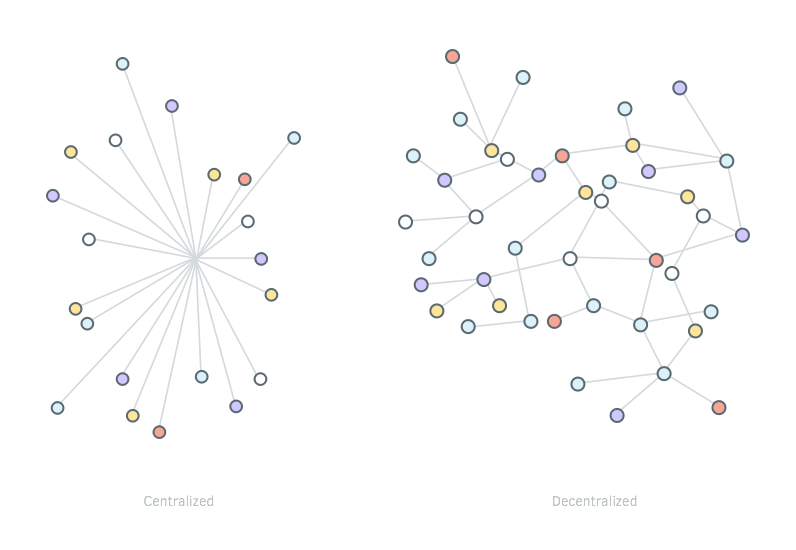
\includegraphics[width=\textwidth]{decentralization.png}
	\caption{Zentrales und dezentrales Netzwerk. Quelle: cryptocoin20.com}
	\label{fig:dencentralized}
\end{figure}

Folgend wird erläutert wie in einer Blockchain die Transaktionen in die Blockchain eingebettet werden. Anschließend wird der Aufbau eines Blockes erläutert. Daraufhin folgt die Erläuterung der Konsensbildung der Blockchain.

\subsection{Transaktionsablauf}
\label{subsec:transaktionsablauf}
Eine Transaktion ist eine Arbeitseinheit, welche eine bestimmte Funktion erf{\"u}llt. In Bezug auf Datenbanksysteme bezeichnet eine Transaktion eine Folge von Datenverarbeitungsbefehlen, die vom System atomar ausgef{\"u}hrt werden.\footnote{\cite[S.~301]{Kemper.2006}} Im Kontext der Blockchain bezeichnet eine Transaktion die Persistierung von Daten, wie beispielsweise einer {\"U}berweisung von Person a zu Person b.\footnote{\cite[S.~2]{SatoshiNakamoto.}} Abbildung \ref{fig:transaktionsablauf} beschreibt den einfachen Transaktionsablauf einer Blockchain.

\begin{figure}[h]
	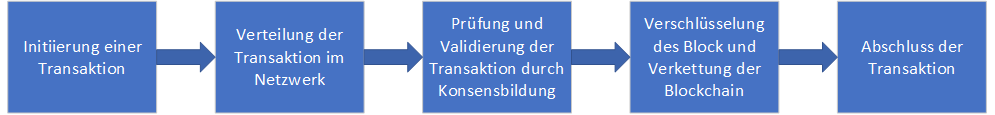
\includegraphics[width=\textwidth]{transaktions-ablauf.png}
	\caption{Vereinfachter Transaktionsablauf. Quelle: Fraunhofer FIT}
	\label{fig:transaktionsablauf}
\end{figure}

Zunächst wird die durchzuführende Transaktion im Netzwerk verteilt. Anschließend fassen die Netzwerkteilnehmer mehrere Transaktionen zu einem Block zusammen und versuchen durch eine Konsensbildung die Transaktionen zu validieren. Die Validierung findet bei der Blockchain-Technologie mit dem sogenannten Proof-Of-Work statt, welche es fordert das aus den Transaktionen und dem vorherigen Block ein Hash mit einer bestimmten Voraussetzung gebildet wird (beispielsweise zehn führende Nullen). Nachdem ein Netzwerkteilnehmer einen validen Hash ermittelt hat, wird der Block an die Kette angehangen und anschließend die veränderte Kette im Netzwerk verteilt. Alle anderen Teilnehmer überprüfen die Erweiterung der Kette mithilfe einer Validierung der Blockhashs. Die Nodes überprüfen auch ob eine Transaktion schon in mehreren Blöcken vorhanden ist oder nicht. Je nach Ergebnis der Validierung wird anschließend die neue Blockchain angenommen oder abgelehnt und die Anpassungen zurückgesetzt.\footnote{\cite[S.~2-4]{SatoshiNakamoto.}}


\subsection{Blockaufbau}
\label{subsec:blockaufbau}
Grundsätzlich besteht ein Block einer Blockchain aus den Transaktionen und Informationen über den aktuellen Block. Mithilfe der Merkle-Root wird aus den einzelnen Transaktionen ein Hashwert ermittelt, jener anschließend in Kombination mit dem vorherigen Blockhash und der freiwählbaren Nonce den Hash des aktuellen Blockes bildet. Mithilfe dieser Einbindung des vorherigen Hash wird die Kette fest miteinander verbunden und die Integrität der Blockchain gewährleistet. In Abbildung \ref{fig:blockaufbau} ist ein Schema der verketteten Blöcke dargestellt.

\begin{figure}[!h]
	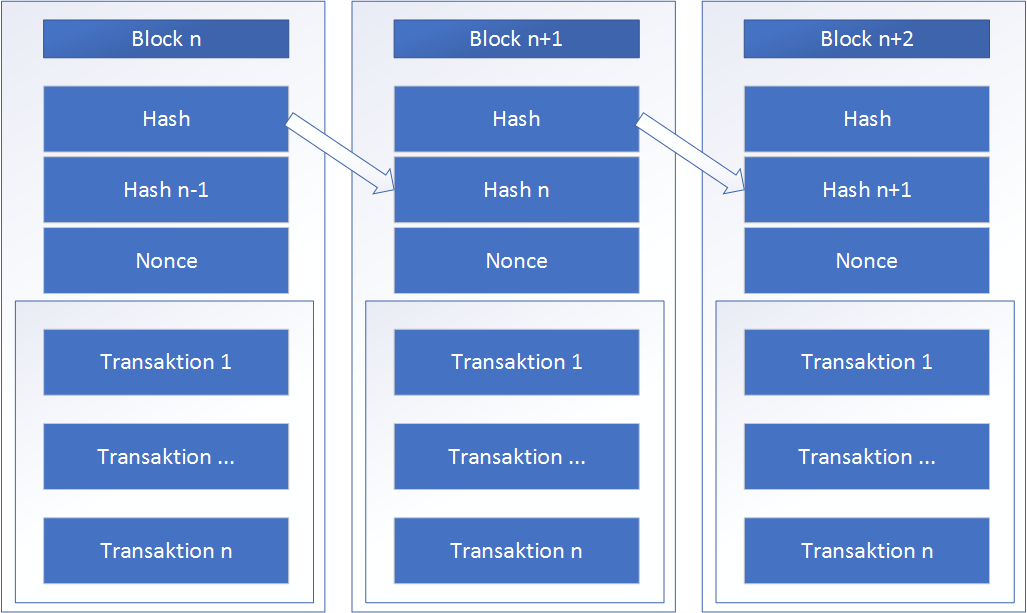
\includegraphics[width=\textwidth]{blockaufbau.png}
	\caption{Blockaufbau. Quelle: Satoshi Nakamoto}
	\label{fig:blockaufbau}
\end{figure}

Die Merkle-Root oder auch Hash-Baum wird für die Sicherstellung der Integrität der Transaktionen verwendet. In Abbildung \ref{fig:hash-tree} ist eine Merkle-Root dargestellt. Zunächst werden alle Transaktionen gehasht. Daraufhin werden zwei gehashte Transaktionen erneut gehasht. Diese Ergebnisse werden anschließend erneut in Zweierpärchen gehasht. Dieser Vorgang wird solange wiederholt, bis nur noch ein Hash übrig ist. Das Ergebnis dieses Verfahren wird als Top-Hash bezeichnet und fließt anschließend in den Blockhash mit ein.\footnote{\cite[S.~4]{SatoshiNakamoto.}}

\begin{figure}[!h]
	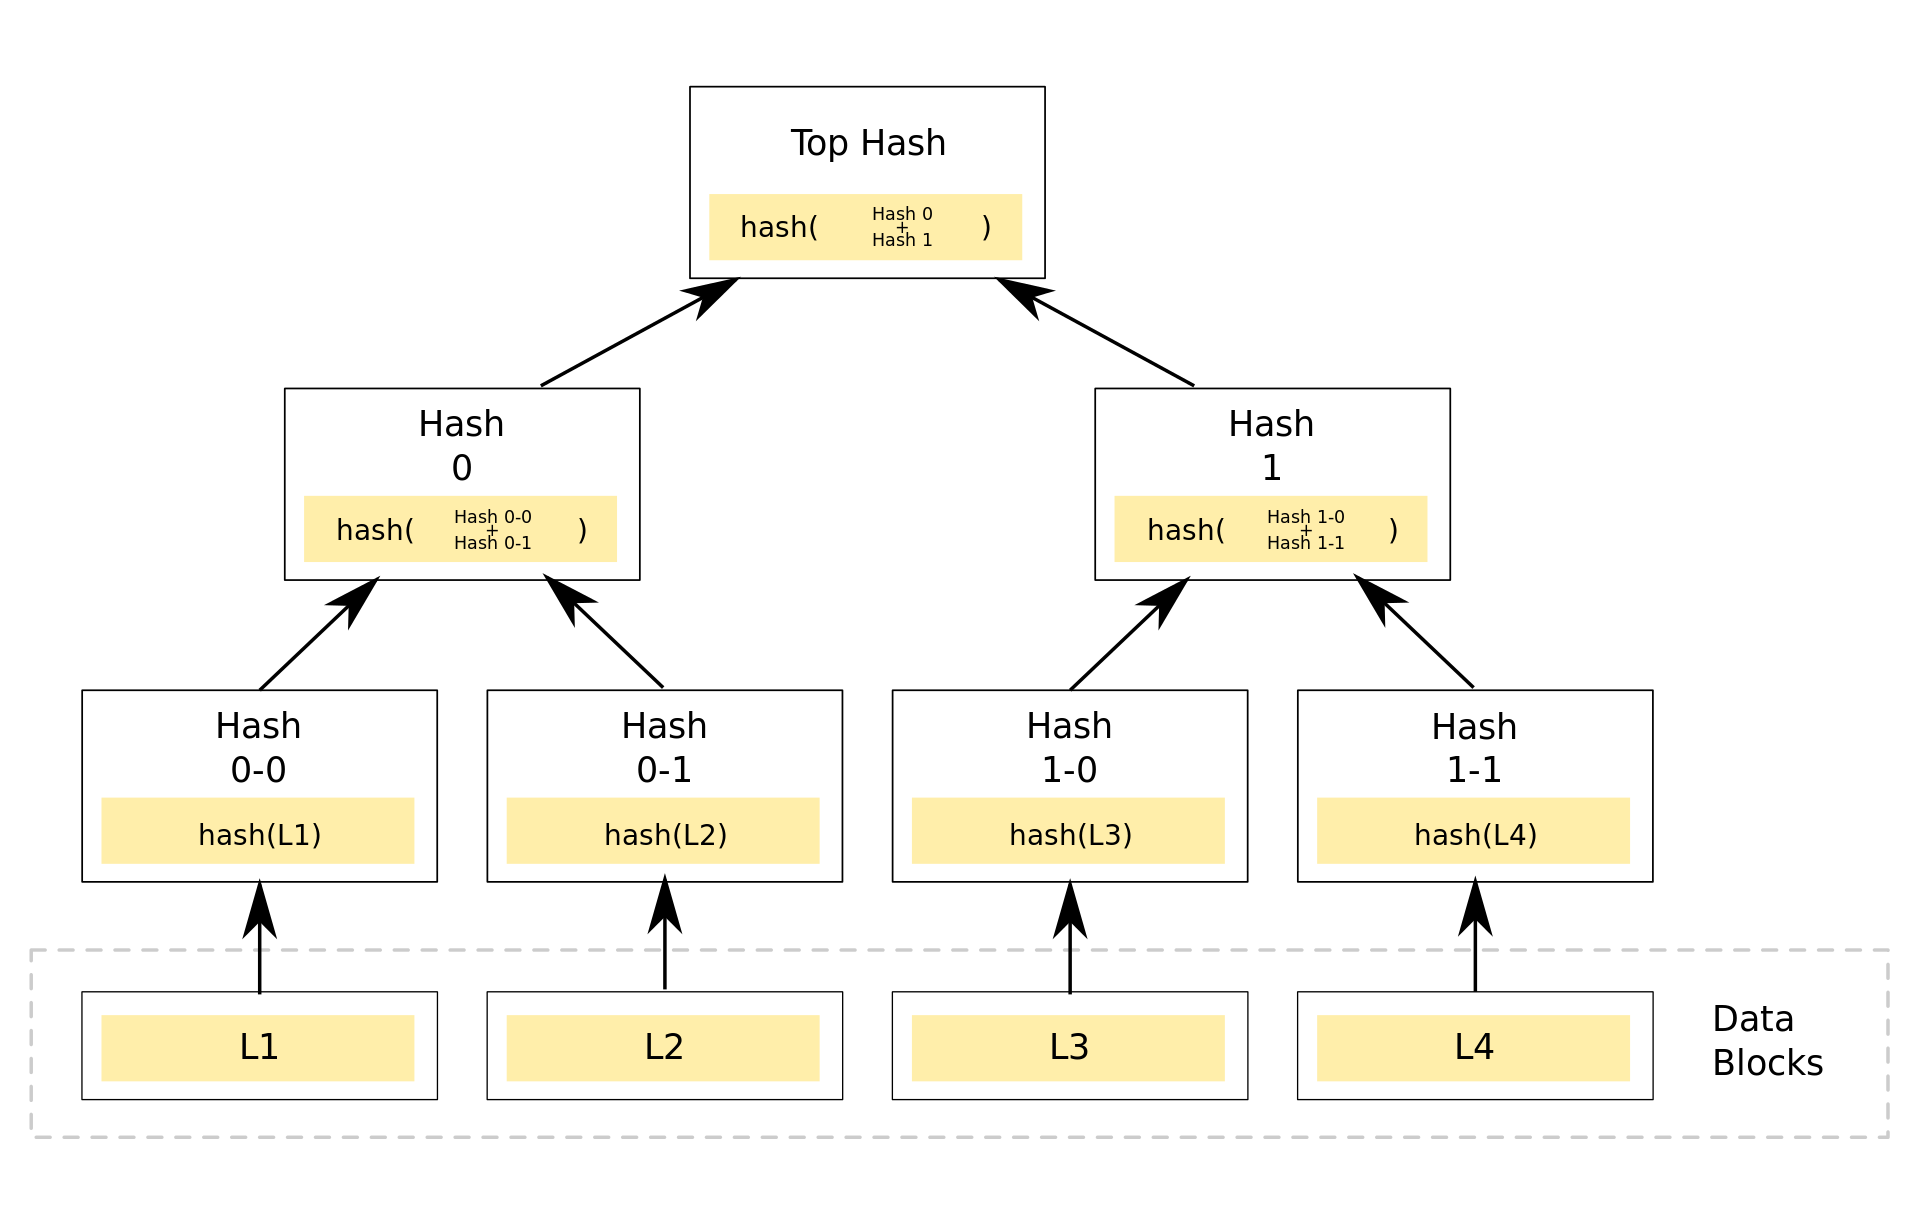
\includegraphics[width=\textwidth]{Hash_Tree.png}
	\caption{Hash-Baum. Quelle: David Göthberg}
	\label{fig:hash-tree}
\end{figure}

\subsection{Konsensbildung}
\label{subsec:Konsensbildung}
Einer der wesentlichen Aspekte des Blockchain-Konzeptes ist die Konsensbildung. Hierbei soll ein Netzwerkteilnehmer beweisen können, dass er berechtigt ist die Blockchain anpassen zu dürfen. Für alle anderen Teilnehmer soll dieser Beweis einfach validierbar sein. Ein weiterer Punkt der Konsensbildung ist die vereinheitlichte Anpassung während der Benutzung der Blockchain. Im den folgenden Kapiteln werden die beiden relevanten Varianten der Konsensbildung vorgestellt.

\subsubsection{Proof-Of-Work}
\label{subsec:proofofwork}
Für Kryptowährungen wird überlicherweise die Proof-Of-Work Variante genutzt. Hierbei muss ein Teilnehmer Arbeit aufwenden, welche anschließend von den anderen Teilnehmern überprüft werden kann.\footnote{\cite[S.~314]{Neugebauer.2018}}

Für die Bitcoin Blockchain müssen beispielsweise Blockhashs mit einer spezifischen Anzahl von führenden Nullen generiert werden. Da eine Hashfunktion eine Einwegfunktion ist, bleibt dem Teilnehmer nichts anderes übrig, als solange den freiwählbaren Teil des Blockes, also den Nonce, anzupassen und anschließend die Hashfunktion auszuführen, bis der gewünschte Hash vorhanden ist.\footnote{\cite[S.~314]{Neugebauer.2018}}

In einer Kryptowährung wie Bitcoin wird in diesem Schritt auch eine Ausschüttung der Währung durchgeführt. Das bedeutet der Teilnehmer, der als erstes die Konsensbildung löst, erhält einen definierten Betrag von der Kryptowährung. Da jedoch mit steigender Nachfrage auch die Anzahl der Netzwerkteilnehmer, bei einer Kryptowährung auch als Miner bezeichnet, steigt, sinkt gleichzeitig die Dauer der Blockerstellung. Um dieser Entwicklung entgegenzuwirken besteht die Möglichkeit die Anforderung an die Konsensbildung regelmäßig zu steigern und somit den steigenden Rechenleistungen entgegenzuwirken.\footnote{\cite[S.~315]{Neugebauer.2018}}

Die Proof-Of-Work Variante ist für öffentliche Blockchains geeignet, da es keine verifizierte Teilnehmer benötigt und trotzdem die Integrität der Blockchain gewährleistet.

\subsubsection{Proof-Of-Stake}
\label{subsec:proofofstake}
Für private Blockchains dagegen ist es nicht immer sinnvoll CPU-Ressourcen für die Konsensbildung zu nutzen. Eine Alternative hierfür wäre das Proof-Of-Stake Verfahren. Hierbei haben einige Nodes besondere Berechtigungen die Blockchain anzupassen und es wird per Zufall ausgewählt, welcher Teilnehmer die Transaktionen an die Blockchain anhängen soll. Die Nodes mit der Berechtigung neue Blöcke an die Blockchain anzuhängen, müssen jedoch in dieser Variante zuvor definiert werden und damit entfällt auch die Unabhängigkeit von einer zentralen Instanz.\footnote{\cite[S.~315--316]{Neugebauer.2018}}

\subsection{Zusammenfassung}
Eine Blockchain ist eine verkette Liste von Blöcken in einem verteilten Peer-To-Peer Netzwerk. Jeder Netzwerkteilnehmer besitzt eine komplette Kopie der Datensätze. Um Daten in das Netzwerk einspeisen zu können, muss der Nutzer eine Transaktion per Broadcast an das Netzwerk senden. Die Netzwerkteilnehmer, auch Nodes genannt, bündeln mehrere Transaktionen und führen je nach Blockchaineigenschaften entweder Proof-Of-Work oder Proof-Of-Stake zur Konsensbildung durch. Hierbei werden zunächst die Transaktionen mithilfe eines Hash-Baums zu einem Hash zusammengefasst. Anschließend wird dieser Hash mit dem Hash des vorherigen Blockes kombiniert. Im Falle der Proof-Of-Work Variante wird danach ein Nonce-Wert gesucht, welcher in Kombination mit den anderen Hashs einen Hash ergibt, der den Ansprüchen der Blockchain genügt. Im Falle der Proof-Of-Stake-Variante wird einfach der Top-Hash der Transaktionen mit dem vorherigen Blockhash kombiniert. Anschließend wird in beiden Verfahren die erweiterte Blockchain im Netzwerk verteilt. Jeder andere Teilnehmer validiert daraufhin die Blockchain.

Da die Blockchain dezentral aufgebaut ist, ergibt sich ein niedriges Ausfallrisiko. Ein weiterer Vorteil der Dezentralität ist das es keine Vertrauensinstanz existieren muss und durch den Proof-Of-Work trotzdem die Integrität der Daten gesichert ist. Eine Blockchain eignet sich aus diesen Gründen für eine öffentliche Währung. Jedoch können Blockchains auch in Unternehmen verwendet werden, da Daten manipulationssicher gespeichert werden können. Diese Eigenschaft könnte beispielsweise in der Rückverfolgung von Lebensmitteln genutzt werden.
% !TEX root = ../document.tex
\section{Blockchain in der Praxis am Beispiel Multichain}
\label{sec:Praxis}
Im nun folgenden Praxisteil soll eine Blockchain aufgesetzt, verwaltet und mit dieser verschiedene Aktionen durchgeführt werden, die einige im Theorieteil vorgestellten Aspekte praktisch vorführen.

\subsection{Installation, Einrichtung und Generierung der Blockchain}
\label{subsec:inst}
Zur Realisation des Praxisteils wird MultiChain verwendet. MultiChain ist eine offene Software mit deren Hilfe schnell und einfach Blockchains erstellt und verwaltet werden können.\footnote{https://www.multichain.com/} Zudem bietet MultiChain einen eigens entwickelten Web-Explorer, um die Blockchain leichter nachvollziehen zu können.\footnote{https://github.com/MultiChain/multichain-explorer} Um die Dezentralität der Blockchain darzustellen, müssen mindestens zwei Nodes die Blockchain verwenden. Um dies allerdings auf einem Computer realisieren zu können und um den Stand des Praxisteils exportierbar zu machen, wird der Praxisteil mit Hilfe zweier virtueller Maschinen verwirklicht. Auf der ersten virtuellen Maschine wird die Blockchain erstellt (im Folgenden Server genannt), sodass die andere virtuelle Maschine (im Folgenden Client genannt) sich dieser Blockchain später anschließen kann.

Um die Blockchain nun auf dem Server einzurichten, muss zunächst MultiChain installiert werden. MultiChain ist sowohl für Linux als auch für Windows und Mac verfügbar. Da beide virtuellen Maschinen allerdings eine Linux-Distribution (Ubuntu) besitzen, wird lediglich auf die Installation für Linux eingegangen. Dazu muss zunächst von der MultiChain-Webseite eine Datei mit den Sourcen heruntergeladen werden, die dann entpackt werden muss. Um MultiChain einfach über das Terminal bedienbar zu machen, werden zudem drei Dateien in den Ordner /usr/local/bin verschoben. Diese Schritte können einfach mittels folgender Zeilen im Terminal durchgeführt werden\footnote{https://www.multichain.com/download-install/}:

\begin{lstlisting}[frame=single]
su (enter root password)
cd /tmp
wget https://www.multichain.com/download/multichain-1.0.4.tar.gz
tar -xvzf multichain-1.0.4.tar.gz
cd multichain-1.0.4
mv multichaind multichain-cli multichain-util /usr/local/bin
exit
\end{lstlisting}

Nachdem MultiChain nun installiert ist, kann die Blockchain erstellt werden. Jede Blockchain muss zudem benannt werden. Für dieses Praxisbeispiel wird die Blockchain „db“ genannt. Mittels folgenden Kommandos kann die Blockchain erstellt werden.

\begin{lstlisting}[frame=single]
multichain-util create db
\end{lstlisting}

Dadurch wird in dem Verzeichnis ~/.multichain nun ein neuer Ordner mit dem Namen der Blockchain angelegt, der die gesamte Blockchain inklusive Daten und Einstellungen enthält. Als nächstes können, falls gewollt, die Parameter der Blockchain angepasst werden. Diese befinden sich in der Datei params.dat des jeweiligen Blockchain-Ordners und können in diesem Fall mittels folgenden Kommandos bearbeitet werden.

\begin{lstlisting}[frame=single]
sudo nano ~/.multichain/db/params.dat
\end{lstlisting}

Eine Liste aller verfügbaren Parameter und deren Bedeutung befindet sich ebenfalls auf der Webseite von MultiChain.\footnote{https://www.multichain.com/developers/blockchain-parameters/} Erwähnenswert in Bezug auf Kryptowährungen ist hier der Parameter initial-block-reward mittels dessen eingestellt werden kann, wie viel Währung ein Node als Belohnung für das erfolgreiche Validieren eines Blocks erhält.

Die Blockchain ist nun erstellt und eingerichtet allerdings noch nicht generiert, d. h. sie besitzt noch keinerlei Blöcke und entsprechend keine Daten. Um die Blockchain nun also zu generieren, muss ein erster Block vom Server validiert werden. Um die Validierung und somit das Errechnen eines gültigen Hashes für den nächsten Block zu starten, wird in diesem (bezogen auf diese Blockchain) folgendes Kommando verwendet.

\begin{lstlisting}[frame=single]
	multichaind db -daemon
\end{lstlisting}

Sobald der erste Block validiert ist, ist die Blockchain generiert.

\subsection{Installation und Einrichtung des MultiChain-Explorers}
\label{subsec:trans-erstellung}
Um die Blockchain auch übersichtlich und verständlich betrachten zu können wird nun der von MultiChain zur Verfügung gestellte Explorer installiert. Die Sourcen für den Explorer befinden sich in einem GitHub-Repository von MultiChain und können (sofern Git auf dem Server installiert ist) mittels folgenden Kommandos heruntergeladen werden:

\begin{lstlisting}[frame=single]
git clone https://github.com/MultiChain/multichain-explorer
\end{lstlisting}

Damit der Explorer lauffähig ist, sind allerdings einige zusätzlichen Programme notwendig, die über folgende Kommandos heruntergeladen und installiert werden können:

\begin{lstlisting}[frame=single]
sudo apt-get install sqlite3 libsqlite3-dev
sudo apt-get install python-dev
sudo apt-get install python-pip
sudo pip install -upgrade-pip
sudo pip install pycrypto
\end{lstlisting}

Als nächstes muss in den nun angelegten Ordner multichain-explorer gewechselt und dort das Skript setup.py mit dem Argument install ausgeführt werden, um den Explorer zu installieren. 

\begin{lstlisting}[frame=single]
cd multichain-explorer
sudo python setup.py install
\end{lstlisting}

Als nächstes muss der Explorer mit der generierten Blockchain kommunizieren können, um die Daten dieser später anzeigen zu können. Jede Blockchain besitzt einen sog. RPC-Port, der in der Datei params.dat im Ordner der Blockchain festgelegt ist. Damit die Blockchain mit dem Explorer kommunizieren kann, wurde bereits beim Erstellen dieser die Datei multichain.conf im Ordner der Blockchain angelegt. In diese Datei muss nun der RPC-Port eingetragen werden. Dies lässt sich einfach über folgende Kommandos realisieren (wobei AUSGEGEBENER\_PORT entsprechend ersetzt werden muss):

\begin{lstlisting}[frame=single]
cd ~/.multichain/db
grep rpc params.dat
echo "rpcport=AUSGEGEBENER_PORT" >> multichain.conf
\end{lstlisting}

Abschließend muss der Explorer noch mit der Blockchain verknüpft werden. Hierzu muss zunächst wieder in den Ordner multichain-explorer navigiert werden. Es muss nun eine Konfigurationsdatei eigens für die erstellte Blockchain angelegt und konfiguriert werden. MultiChain-Explorer bietet hierzu eine vorgefertigte Konfigurationsdatei (chai1.example.conf) die einfach kopiert und unter dem Namen der Datenbank (db.conf) gespeichert werden kann. Innerhalb der Datei können bzw. müssen nun folgende Parameter eingestellt werden:

\begin{table}[h]
	\begin{tabular}{|l|l|}
		\hline 
		\textbf{Parameter} & \textbf{Beschreibung} \\ 
		\hline 
		port & Port, über den die Seite im Browser erreichbar sein soll \\ 
		\hline 
		host & IP des Gerätes, das den Explorer aufrufen können soll (0.0.0.0 für alle Geräte) \\ 
		\hline 
		dirname & Absoluter Pfad zum Ordner der Datenbank (hier: ~/.multichain/db) \\ 
		\hline 
		chain & Name der Blockchain, der im Explorer angezeigt werden soll \\ 
		\hline 
		connect-args & Speicherort der Explorer-Datenbank (hier: db.explorer.sqlite) \\ 
		\hline 
	\end{tabular}
	\caption{Konfigurierbare Parameter der Explorer-Blockchain-Verbindung}
\end{table}

Nachdem die Parameter entsprechend angepasst wurden, kann die Datei mit der Tastenkombination STRG + X verlassen werden, wobei auf die Nachfrage, ob die Änderungen gespeichert werden sollen mit Y + Enter und danach der Dateiname mit Enter bestätigt werden müssen.

Nun kann der Explorer mit folgendem Kommando gestartet werden:

\begin{lstlisting}[frame=single]
sudo python -m Mce.abe -config db.conf
\end{lstlisting}

Der Explorer liest dann zunächst die bislang getätigten Transaktionen und validierten Blöcke in die eigene Datenbank ein. Der Explorer kann dann über die Adresse des Servers und dem angegebenen Port aufgerufen werden (s. Abbildung \ref{fig:1}).

\begin{figure}[h]
	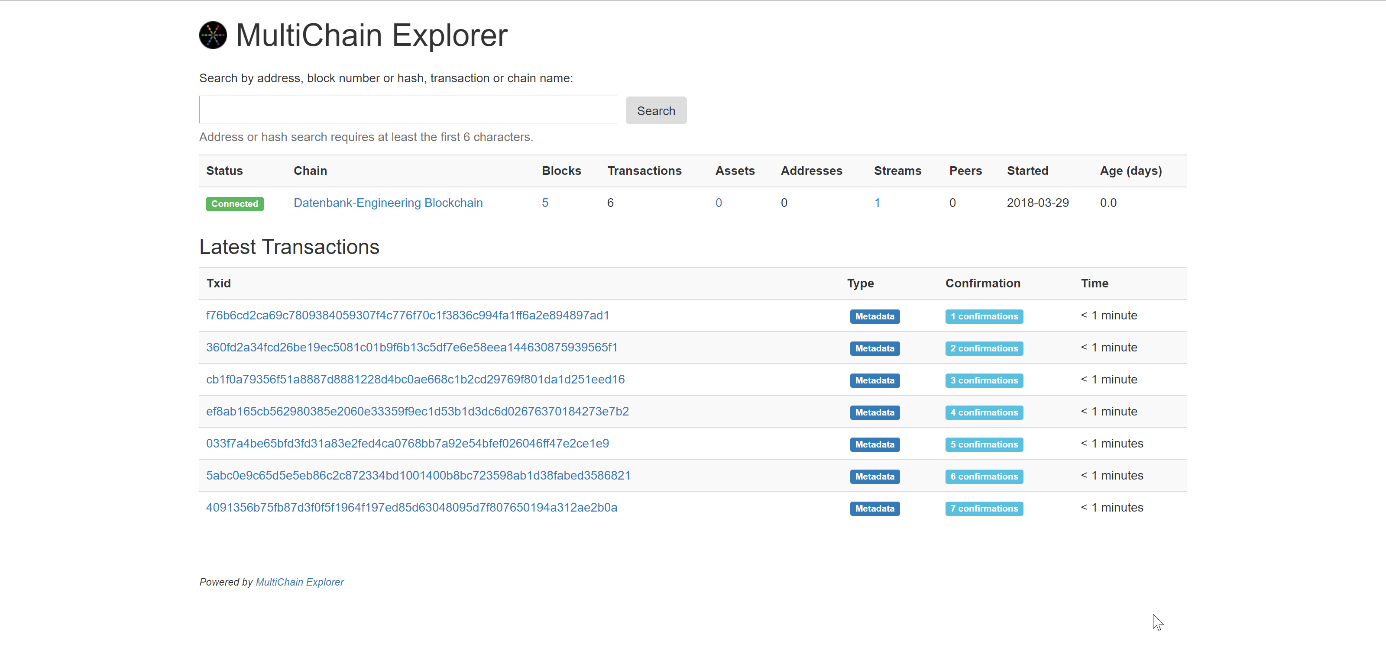
\includegraphics[width=\textwidth]{1.png}
	\caption{Startseite des Explorer}
	\label{fig:1}
\end{figure}

\subsection{Anbinden eines zweiten Knoten an die Blockchain}
\label{subsec:trans-erstellung-mit-daten}
Um nun unseren Client zum zweiten Knoten der Blockchain zu machen, müssen wir auch auf diesem zunächst MultiChain installieren. Voraussetzung für die Verbindung ist nun, dass sich die beiden Computer (bzw. hier die beiden virtuellen Maschinen) im selben Netzwerk befinden. Als der Server als Knoten der Blockchain gestartet wurde, wurde im Terminal des Servers folgendes ausgegeben:

\begin{figure}[h]
	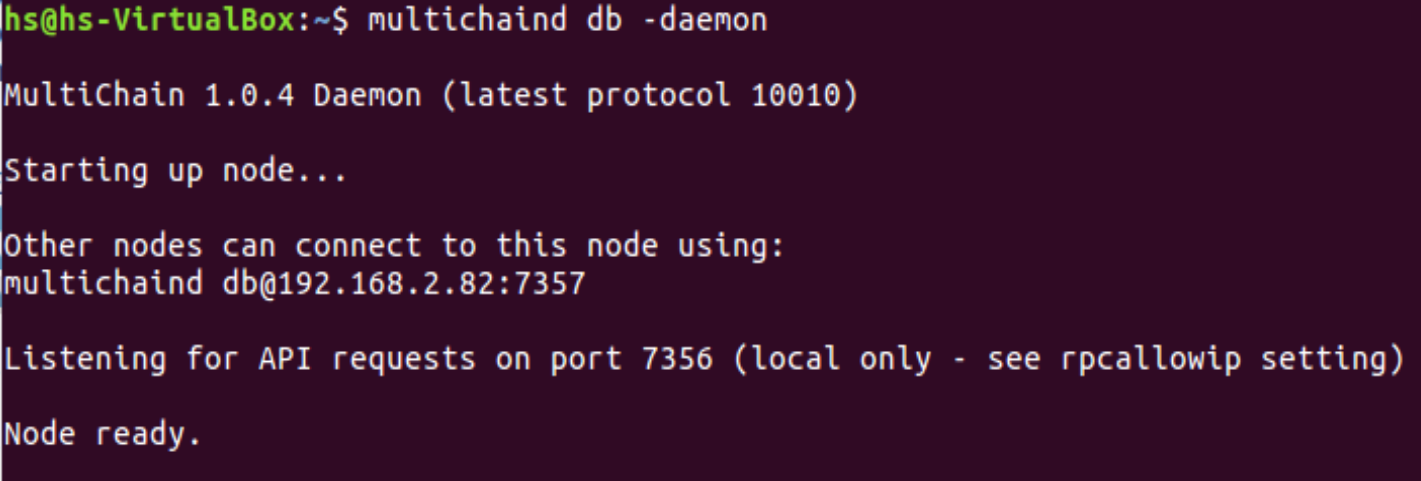
\includegraphics[width=\textwidth]{2.png}
	\caption{Ausgabe des Kommandos multichaind db -daemon im Terminal des Servers}
	\label{fig:2}
\end{figure}

Hier wird mitgeteilt, wie man sich mit anderen Computern im selben Netzwerk mit der Blockchain verbinden kann. Dazu muss man lediglich den Befehl multichaind eingeben gefolgt von dem Namen der Blockchain, einem @-Zeichen, der IP des Servers, einem Doppelpunkt und einem gesetzten Port. In diesem Falle setzt sich daraus folgendes Kommando zusammen:

\begin{lstlisting}[frame=single]
multichaind db@192.168.2.82:7357
\end{lstlisting}

Wenn dieses Kommando nun im Terminal des Clients eingegeben wird, erscheint allerdings ein Hinweis, dass Blockchain selbst zwar empfangen und erfolgreich auf dem Client initialisiert wurde, der Client nicht die nötigen Rechte zum Verbinden der Blockchain besitzt.

\begin{figure}[h]
	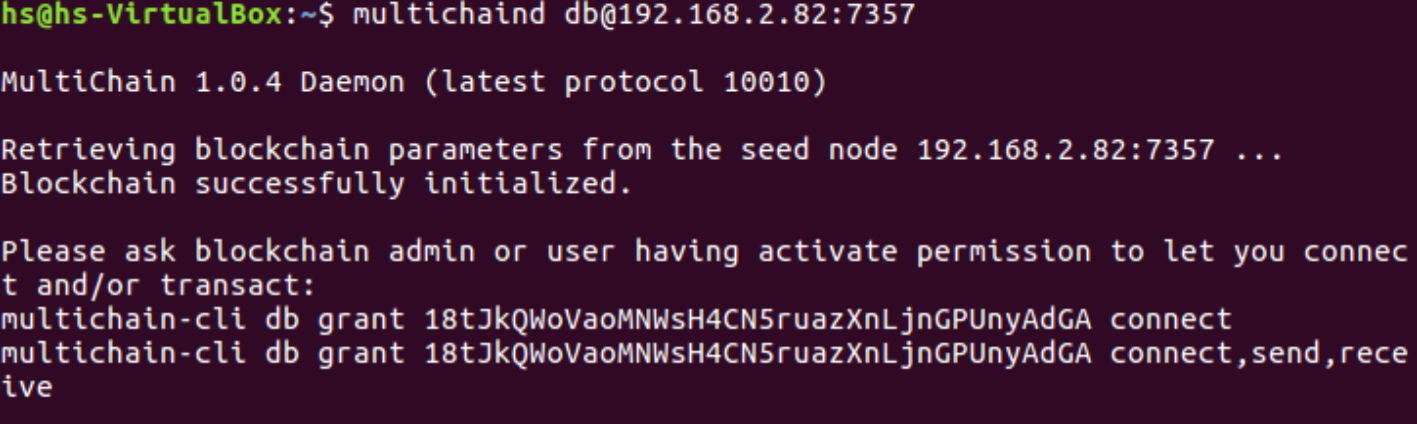
\includegraphics[width=\textwidth]{3.png}
	\caption{Initialisierung der Blockchain auf dem Client}
	\label{fig:3}
\end{figure}

MultiChain stellt eine Blockchain generell so ein, dass sich niemand ohne explizites Recht mit einer Blockchain verbinden kann. Dies kann allerdings vor der Generierung der Blockchain über den Parameter anyone-can-connect in der params.dat der jeweiligen Blockchain angepasst werden. Neben der Meldung über die fehlenden Rechte zeigt das Terminal des Clients allerdings auch direkt das Kommando an, das auf dem Server eingegeben werden muss, um dem Client die Rechte zum Verbinden zu geben:

\begin{lstlisting}[frame=single]
multichain-cli db grant 18tJkQWoVaoMNWsH4CN5ruazXnLjnGPUnyAdGA connect
\end{lstlisting}

Auffällig ist hierbei die lange, zufallsgenerierte Zeichenkette. MultiChain vergibt jedem Knoten eine einzigartige ID und die hier angezeigte ID ist die ID, die für den Client generiert wurde. Nachdem wir das Kommando im Terminal des Servers eingegeben haben, kann sich der Client mit der Blockchain verbinden und als Knoten gestartet werden.

Vorher sollen dem Client allerdings zusätzlich die Rechte zum Validieren von Blöcken und Tätigen von Transaktionen gegeben werden. Dazu wird folgendes Kommando benötigt:

\begin{lstlisting}[frame=single]
multichain-cli db grant 18tJkQWoVaoMNWsH4CN5ruazXnLjnGPUnyAdGA mine,send,receive
\end{lstlisting} 

Bevor der Knoten nun gestartet wird, soll allerdings noch ein Blick in das Verzeichnis ~/.multichain auf dem Client geworfen werden. In diesem befindet sich bereits der Ordner der installierten Blockchain db. Wechselt man in den Ordner der Blockchain und und betrachtet den Inhalt, beinhaltet dieser bereits einige generelle Dateien die Blockchain. Vergleicht man den Ordner allerdings mit demselben Ordner auf dem Server, sieht man, dass der Server sowohl mehr Dateien als auch mehr Ordner beinhaltet. Teilweise sind dies solche, die lediglich der Server als Ersteller der Blockchain besitzt, teilweise sind dies wie z. B. der Ordner wallet allerdings auch die Transaktionen bzw. Daten der Blockchain. 

\begin{figure}[h]
	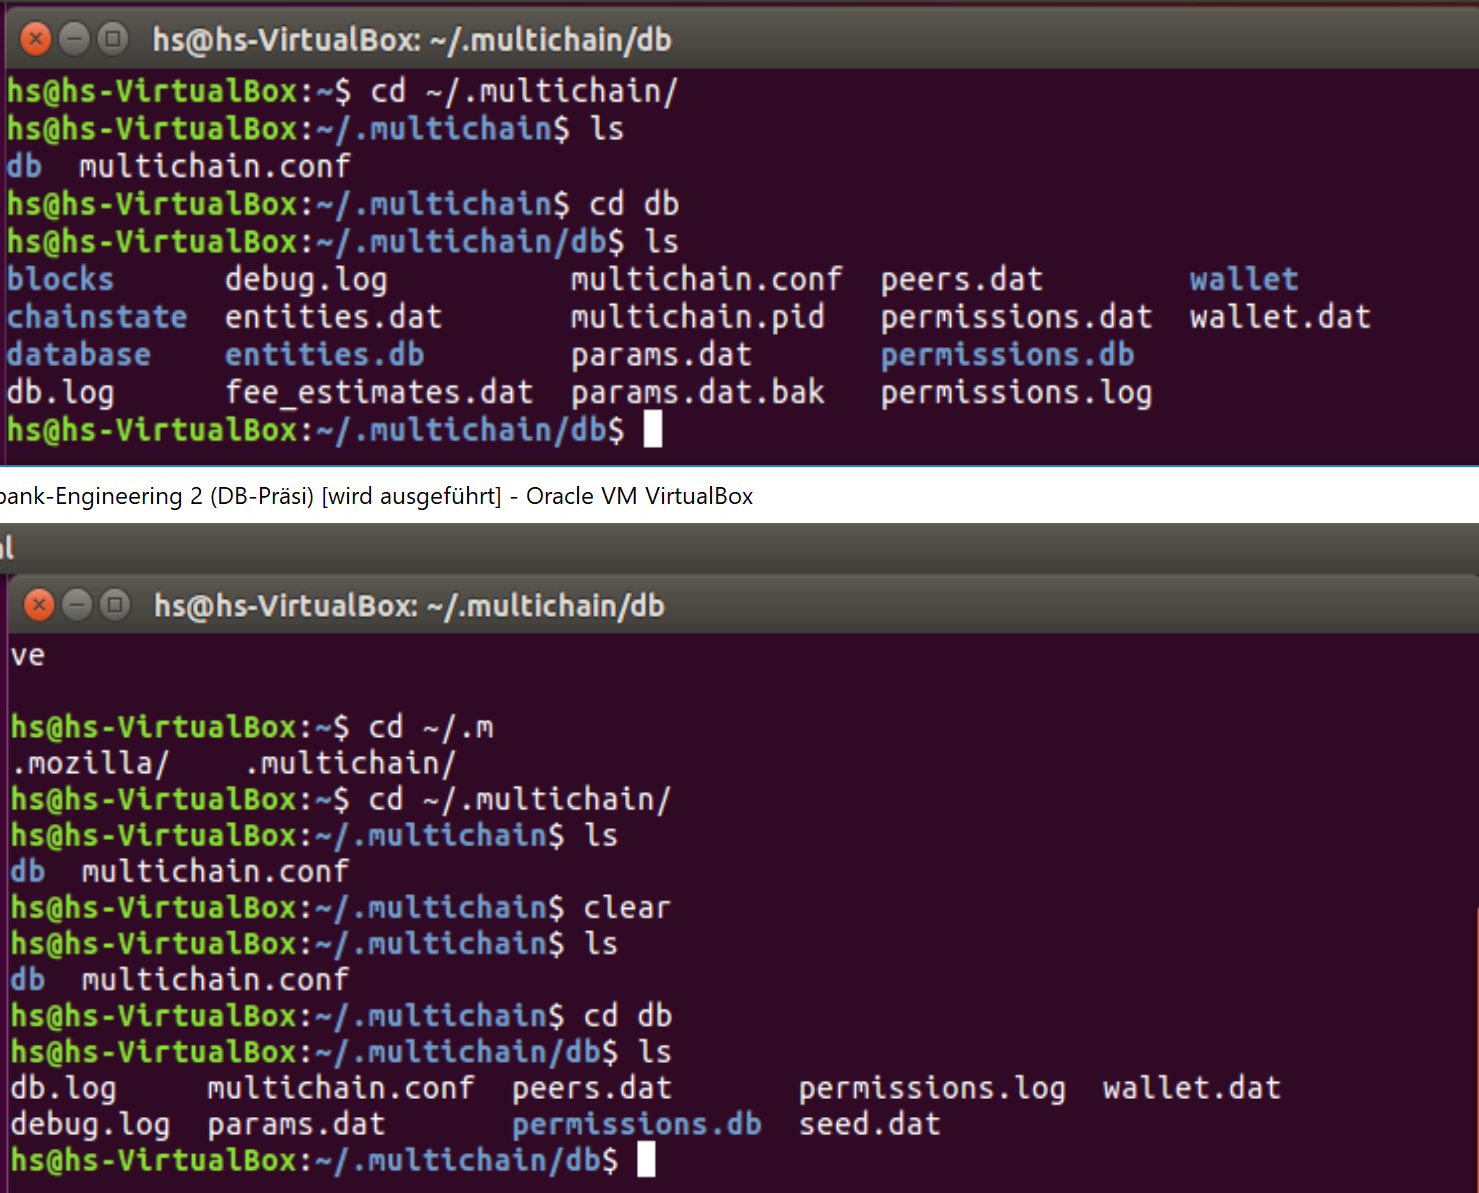
\includegraphics[width=\textwidth]{4.png}
	\caption{Vergleich des ~/.multichain/db-Ordners auf dem Server und dem Client}
	\label{fig:4}
\end{figure}

Um den Client nun als Knoten der Blockchain zu starten, wird dasselbe Kommando wie auf dem Server verwendet (multichaind db -daemon). An dieser Stelle wird nun die Dezentralität der Blockchain hervorgehoben: der Client empfängt nun alle Daten der Blockchain (Blöcke, Transaktionen, …), sodass alle Daten der Blockchain auf beiden Knoten liegen. Betrachtet man bspw. den Ordner wallet wird deutlich, dass beide Knoten alle Transaktionen beinhalten. Sobald neue Transaktionen hinzukommen, erhalten beide Knoten diese.

\begin{figure}[h]
	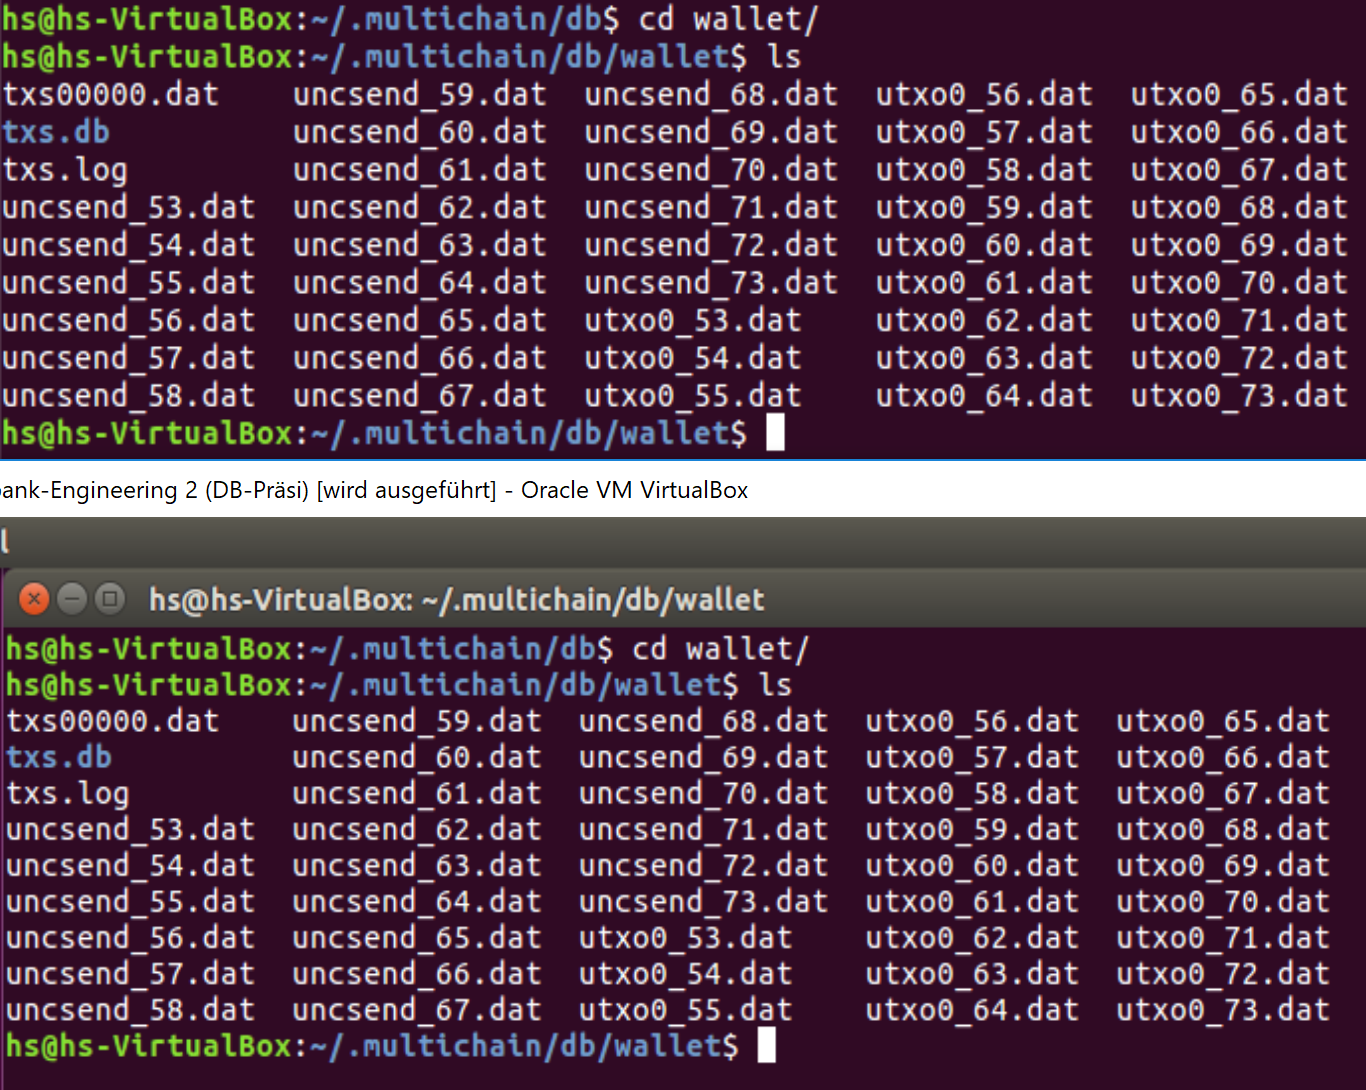
\includegraphics[width=\textwidth]{5.png}
	\caption{Vergleich des wallet-Ordners auf dem Server und dem Client}
	\label{fig:5}
\end{figure}

\subsection{Betrachtung der Blockchain im Explorer}
Beide Knoten sind nun am validieren der Blöcke. Dies lässt sich über den Explorer verfolgen. Wird die Startseite (s. Abbildung \ref{fig:1}) betrachtet, wird die Blockchain mit dem in der Datei db.conf angegebenen Namen angezeigt. Darunter werden zudem die letzten getätigten Transaktionen angezeigt. Wird nun neben dem Namen der Blockchain auf die Anzahl der Blöcke geklickt, gelangt man zur Übersicht der Blöcke der Blockchain (s. Abbildung \ref{fig:6}).

\begin{figure}[h]
	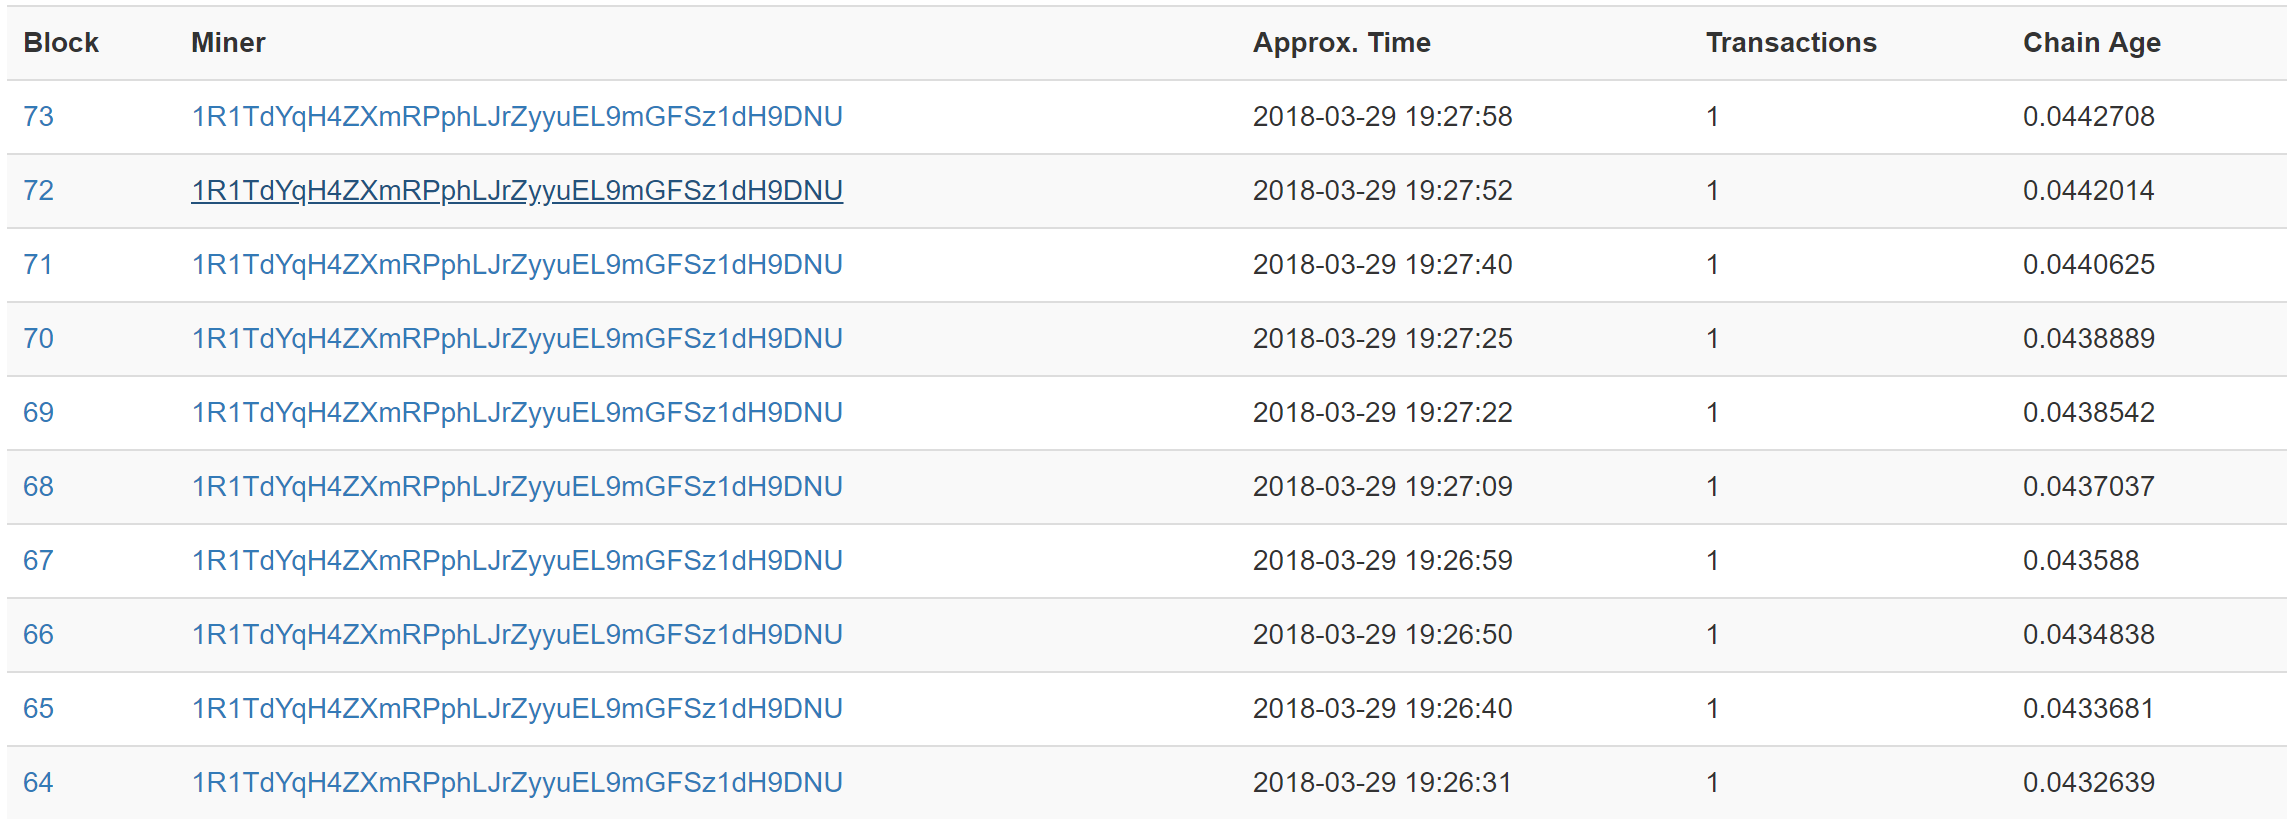
\includegraphics[width=\textwidth]{6.png}
	\caption{Übersicht der Blöcke der Blockchain}
	\label{fig:6}
\end{figure}

In der Liste wird für jeden Block folgendes angezeigt: die Nummer des Blocks in der Blockchain, die ID des Knotens, der diesen Block validiert hat, der Validierungszeitpunkt, die Anzahl der Transaktionen, die der Block beinhaltet bzw. validiert hat und das Alter der Blockchain zum Zeitpunkt der Validierung des Blocks in Tagen. Auffällig ist hierbei, dass die Blöcke bislang alle lediglich eine Transaktion beinhalten. Dies ist darauf zurückzuführen, dass die einzigen Transaktionen, die bislang ausgeführt wurden, die Gewinnausschüttung der Belohnung für das Validieren eines Blockes ist. Wird nun auf die Zahl eines Blocks geklickt, gelangt man zur Übersicht des Blocks (s. Abbildung \ref{fig:7}).

\begin{figure}[h]
	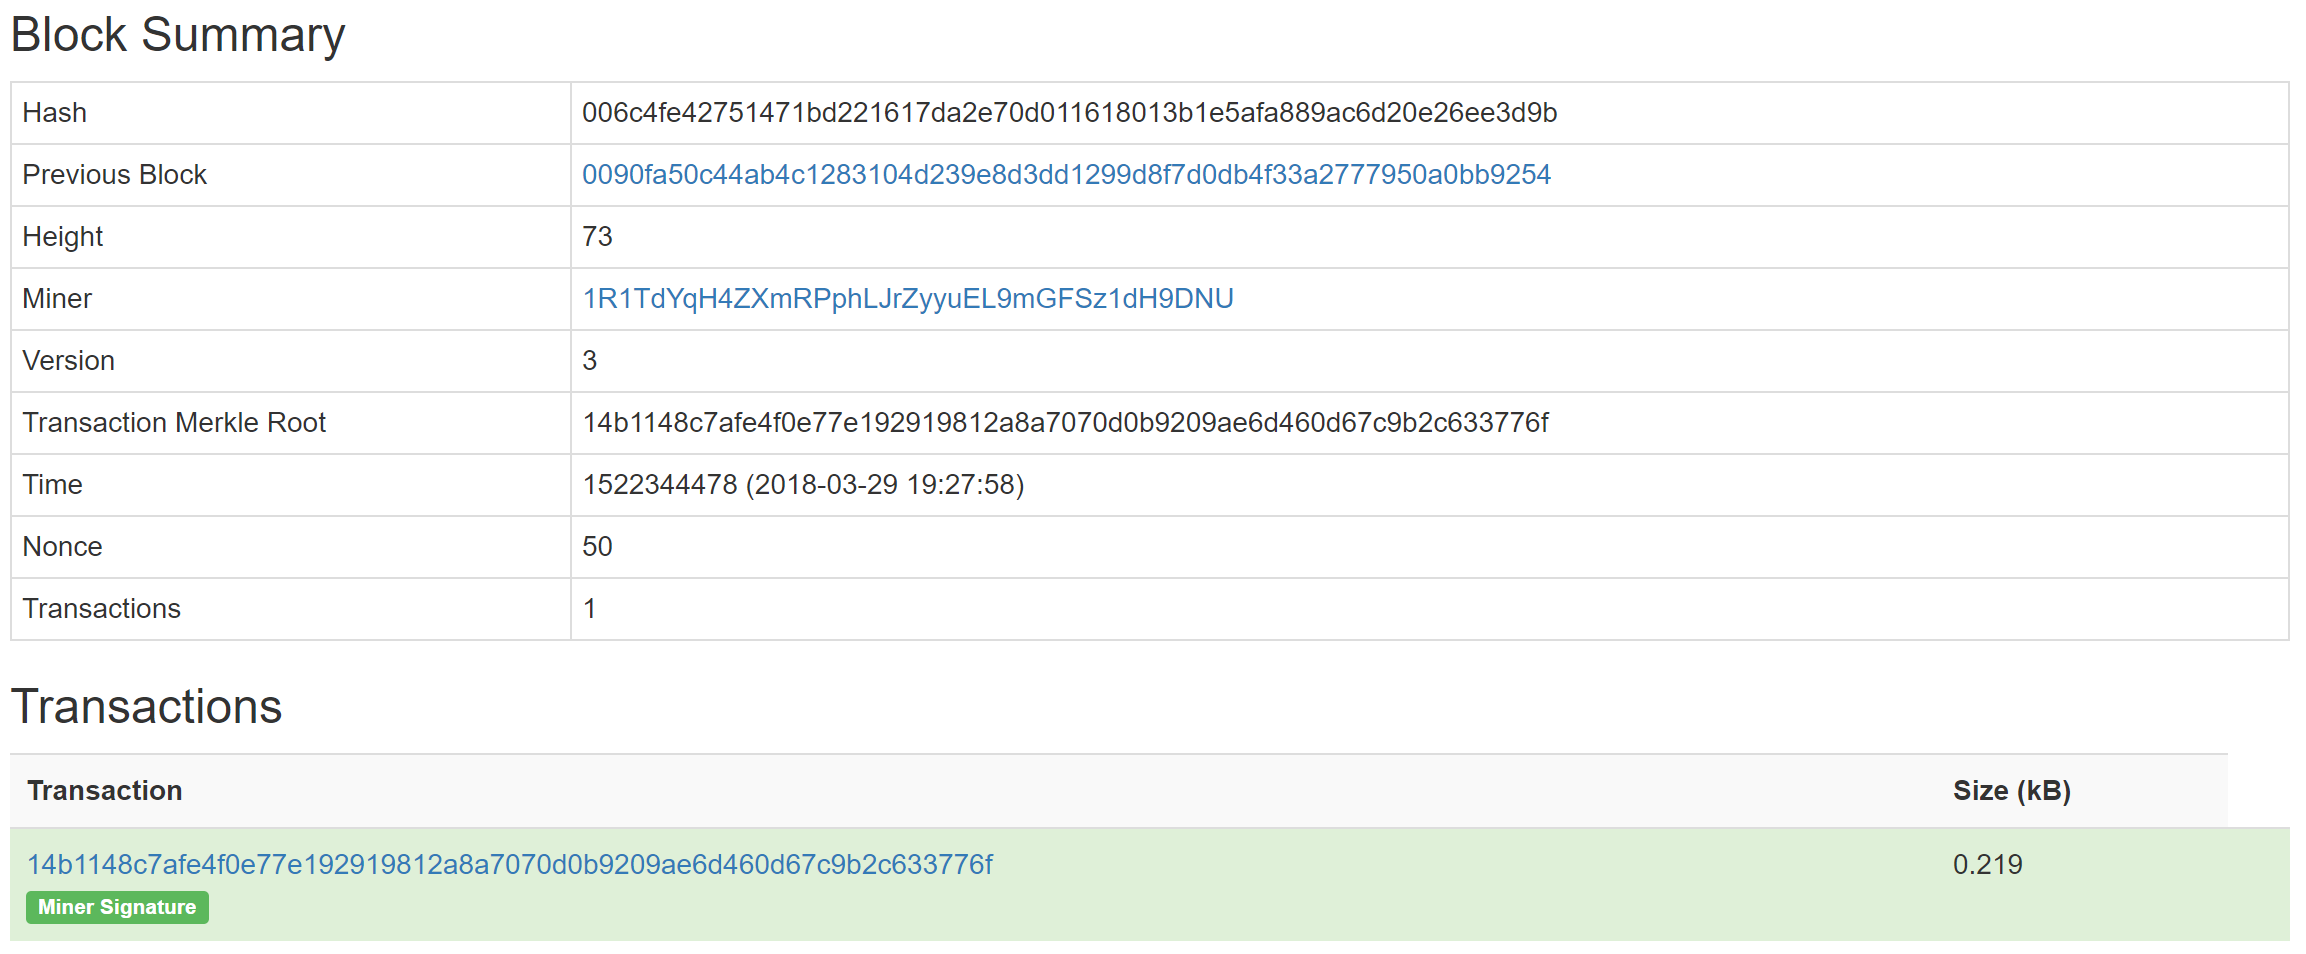
\includegraphics[width=\textwidth]{7.png}
	\caption{Ansicht eines Blocks im Explorer}
	\label{fig:7}
\end{figure}

In der Übersicht sieht man eine Liste mit Eigenschaften des Blocks und darunter die beinhalteten Transaktionen. In der Liste befindet sich zunächst der Hash des Blocks, der als gültiger Hash zum Validieren des Blocks errechnet worden ist. Bei MultiChain-Blockchains ist standardmäßig die Regelung eingestellt, dass ein Hash lediglich gültig ist, wenn er mindestens zwei Nullen voranstehen hat. Des Weiteren beinhaltet die Liste den Hash des vorherigen Blocks. Sobald ein nächster Block validiert wurde, wird zudem der Hash des nächsten Blocks eingetragen. Hier wird deutlich, wie die Blöcke verkettet sind und, dass eine entsprechend durch eine Änderung eines Blockes die Hash-Werte aller folgenden Blöcke neu berechnet werden müssten. Der Wert „Height“ zeigt die Nummer des Blocks in der Blockchain an. Darunter befindet ich die ID des Knotens, der den Block validiert hat. Des Weiteren wird die Transaction Merkle Root angegeben, die zur Errechnung des Hash-Wertes verwendet wurde. Auch der Validierungszeitpunkt und die Anzahl der enthaltenen Transaktionen sind in der Liste aufgeführt. Zuletzt wird auch die Nonce angegeben, die zum Berechnen des Hash-Wertes verwendet wurde. Wird nun auf die ID der enthaltenen Transaktion  geklickt, öffnet sich eine entsprechende Detail-Ansicht, die die Informationen der Transaktion darstellt.

\begin{figure}[h]
	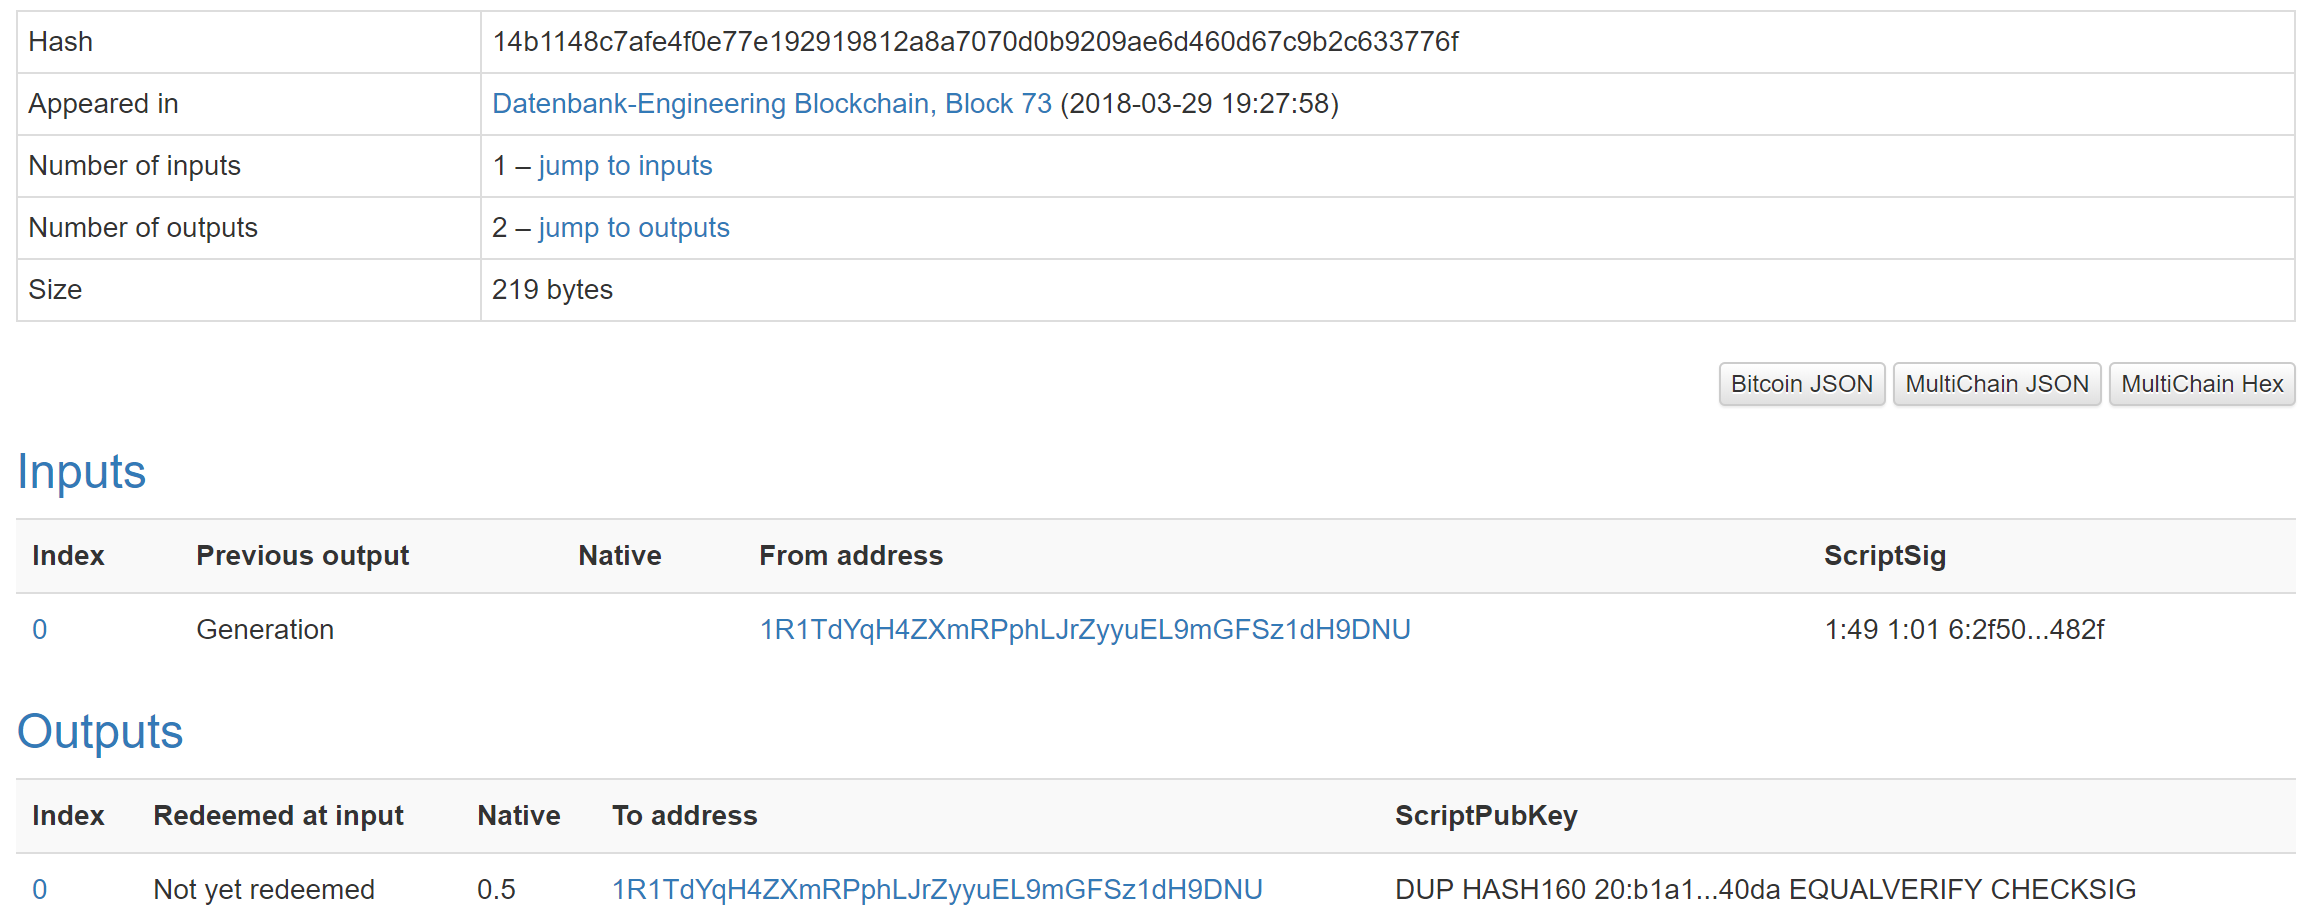
\includegraphics[width=\textwidth]{8.png}
	\caption{Detail-Ansicht einer Transaktion}
	\label{fig:8}
\end{figure}

Diese Ansicht stellt unter anderem den Hash-Wert/die ID der Transaktion, die Nummer des Blocks, in dem sie enthalten ist, und die Größe der Transaktion in Bytes dar. Außerdem sind die Inputs und Outputs der Transaktion dargestellt. Die Inputs stellen dar, wer etwas geschickt hat (From Address), wie sich die geschickte Anzahl an Währung vom Sender zusammenstellt (Native) und woher diese kommt (Previous Input). Im Output wird dargestellt, wer das Ergebnis der Transaktion erhält (To address) und wie viel Währung er erhält (Native). In Falle der abgebildeten Transaktion schickt der Server an sich selbst 0.5 Währung, die neu generiert werden (Previous Output = Generation). Dies ist die Belohnung für das erfolgreiche Validieren eines Blockes. Wird nun auf die ID eines Knotens geklickt, gelangt man zur Ansicht dessen (s. Abbildung \ref{fig:9}):

\begin{figure}[h]
	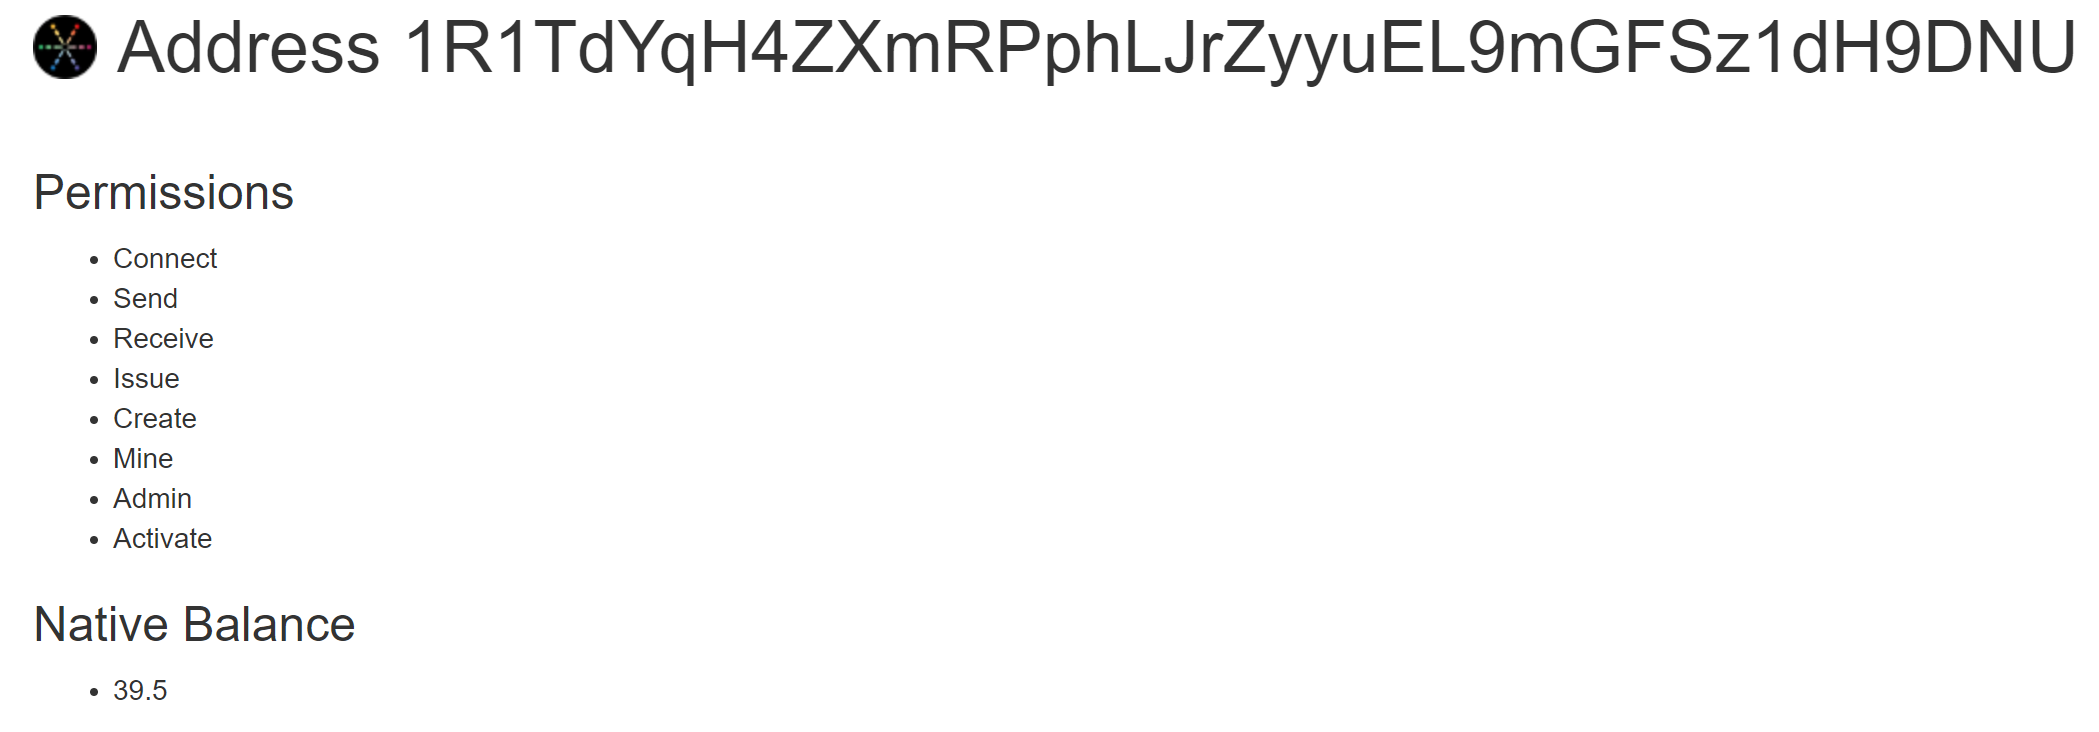
\includegraphics[width=\textwidth]{9.png}
	\caption{Explorer-Ansicht eines Knotens}
	\label{fig:9}
\end{figure}

Hier werden lediglich die Berechtigungen des Knotens (Permissions) und die Anzahl der Währung, die dieser momentan besitzt (Native Balance) aufgeführt.

\subsection{Manuelle Durchführung einer Transaktion}
Um nun eine manuelle Transaktion durchzuführen, kann man zunächst von einem Knoten zum anderen Währung überweisen. Diese Transaktion wird dann zunächst an alle Knoten der Blockchain übermittelt und dann in den nächsten Block mit aufgenommen und durch Validierung dieses Blockes gültig und durchgeführt. Um eine Transaktion von Währung durchzuführen, muss das Kommando multichain-cli gefolgt von dem Namen der Blockchain, dem Befehl send, der ID des Empfänger-Knotens und die zu überweisende Anzahl der Währung eingegeben werden. So könnte eine Überweisung des Servers an den Client wie folgt lauten:

\begin{lstlisting}[frame=single]
multichain-cli db send 18tJkQWoVaoMNWsH4CN5ruazXnLjnGPUnyAdGA 2.0
\end{lstlisting} 

Wird diese Transaktion nun durchgeführt, wird sie auf der Startseite des Explorers aufgeführt ist zunächst allerdings noch nicht bestätigt, da diese noch in keinen validierten Block mit aufgenommen wurde (s. Abbildung \ref{fig:10}).

\begin{figure}[h]
	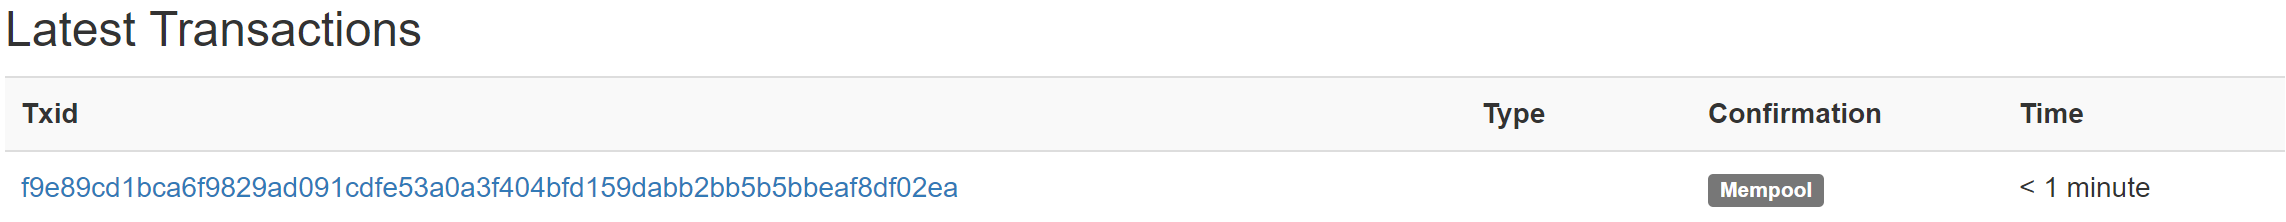
\includegraphics[width=\textwidth]{10.png}
	\caption{Unbestätigte Transaktion des Servers an den Client}
	\label{fig:10}
\end{figure}

Sobald diese Transaktion in einen validierten Block mit aufgenommen wurde, ist sie bestätigt. Wird diese Transaktion nun im Explorer betrachtet (s. nächste Abbildung), sieht man, dass der Server (From Address) viermal 0.5 Währung (Native) verschickt hat und auch aus welchen Transaktionen diese stammen (Previous Output). Dies ist dazu zurückzuführen, dass der Server bislang lediglich mehrmals 0.5 Währung durch das Validieren von Blöcken erhalten hat. Auf der Empfängerseite der Transaktion sieht man allerdings, dass der Client (To address) 2 Währung (Native) erhalten hat.

\begin{figure}[h]
	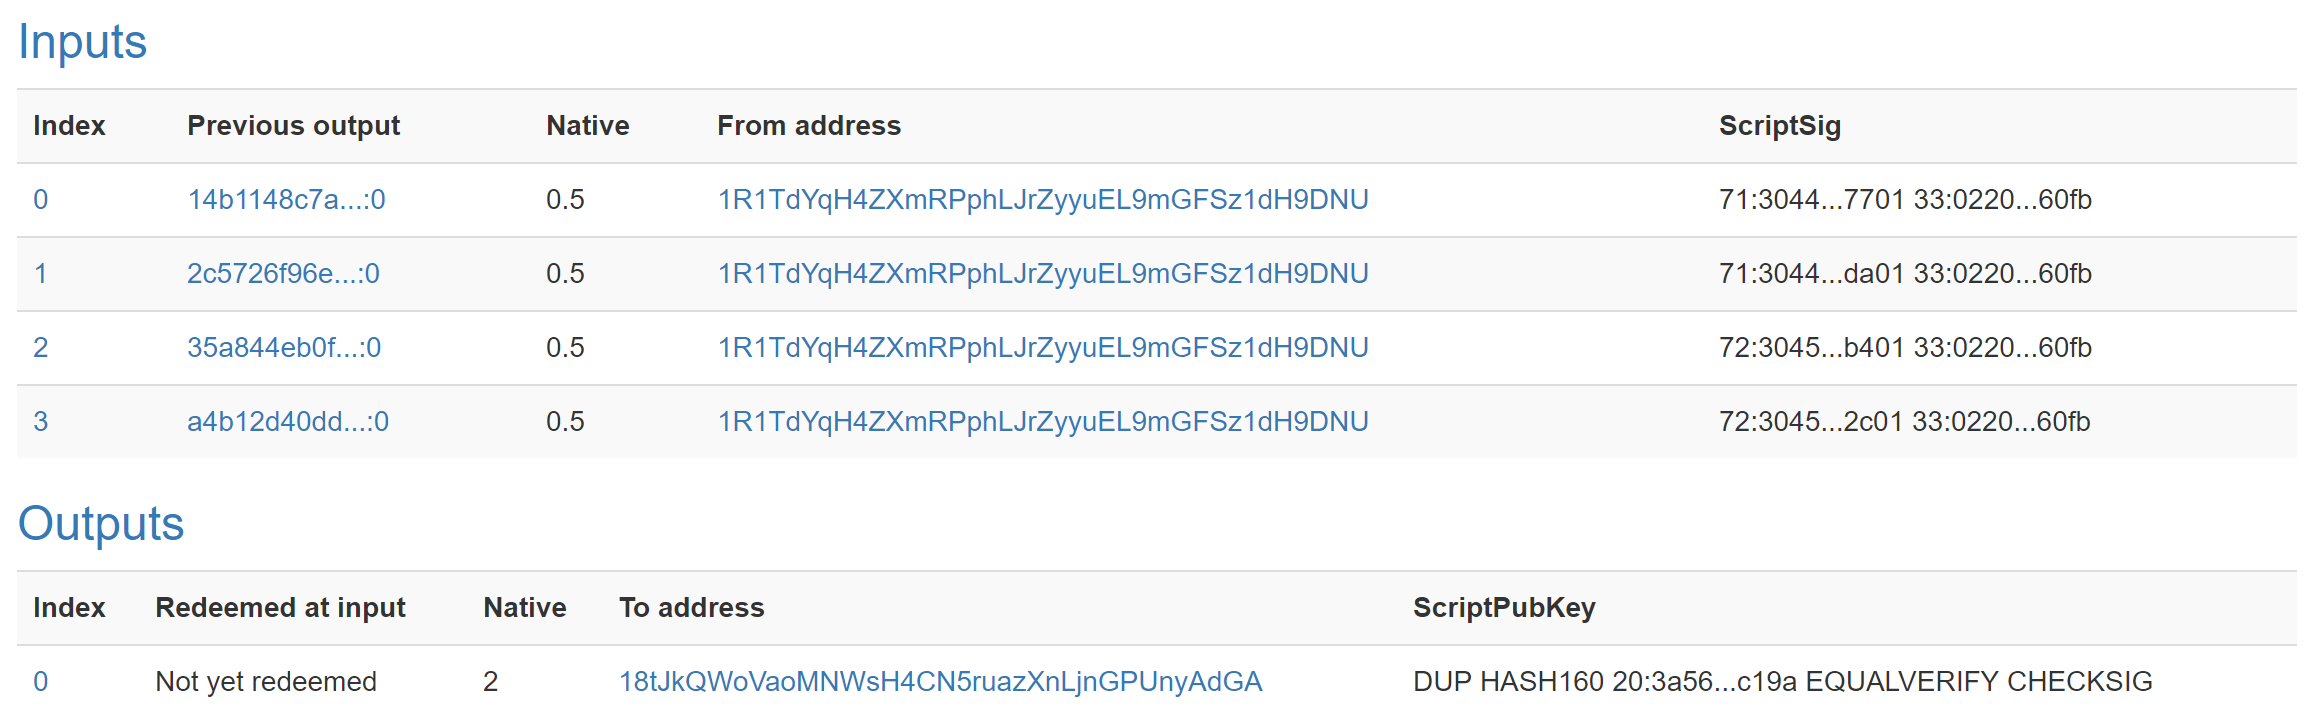
\includegraphics[width=\textwidth]{11.png}
	\caption{Betrachtung der Transaktion des Servers an den Client}
	\label{fig:11}
\end{figure}

\subsection{Speichern von Daten}
Neben dem Verschicken von Währung können in einer Blockchain allerdings auch allgemeine Daten gespeichert werden. Hierzu wird erneut auf das Kommando multichain-cli zurückgegriffen. Dabei muss erneut die Blockchain angegeben werden, gefolgt von dem Befehl publish, einem sog. Stream (root ist der Standard-Stream der Blockchain), einem Key dem die Daten zugeordnet werden sollen und mittels dem später alle Daten abgefragt werden können, die diesem Key jemals in dieser Blockchain zugeordnet wurden und den Daten selbst. Die Daten müssen allerdings im Hexadezimalformat angehängt werden. Dies hat den Vorteil, dass ganze Bilder oder Videos im hexadezimal kodierten Format an die Blockchain angehängt werden können. Ein entsprechendes Kommando könnte für diese Blockchain wie folgt aussehen:

\begin{lstlisting}[frame=single]
multichain-cli db publish key1 12345d
\end{lstlisting} 

Sobald man das Kommando bestätigt, wird eine neue Transaktion angelegt, die die Daten enthält. Die folgende Abbildung stellt diese Transaktion im Explorer dar:

\begin{figure}[h]
	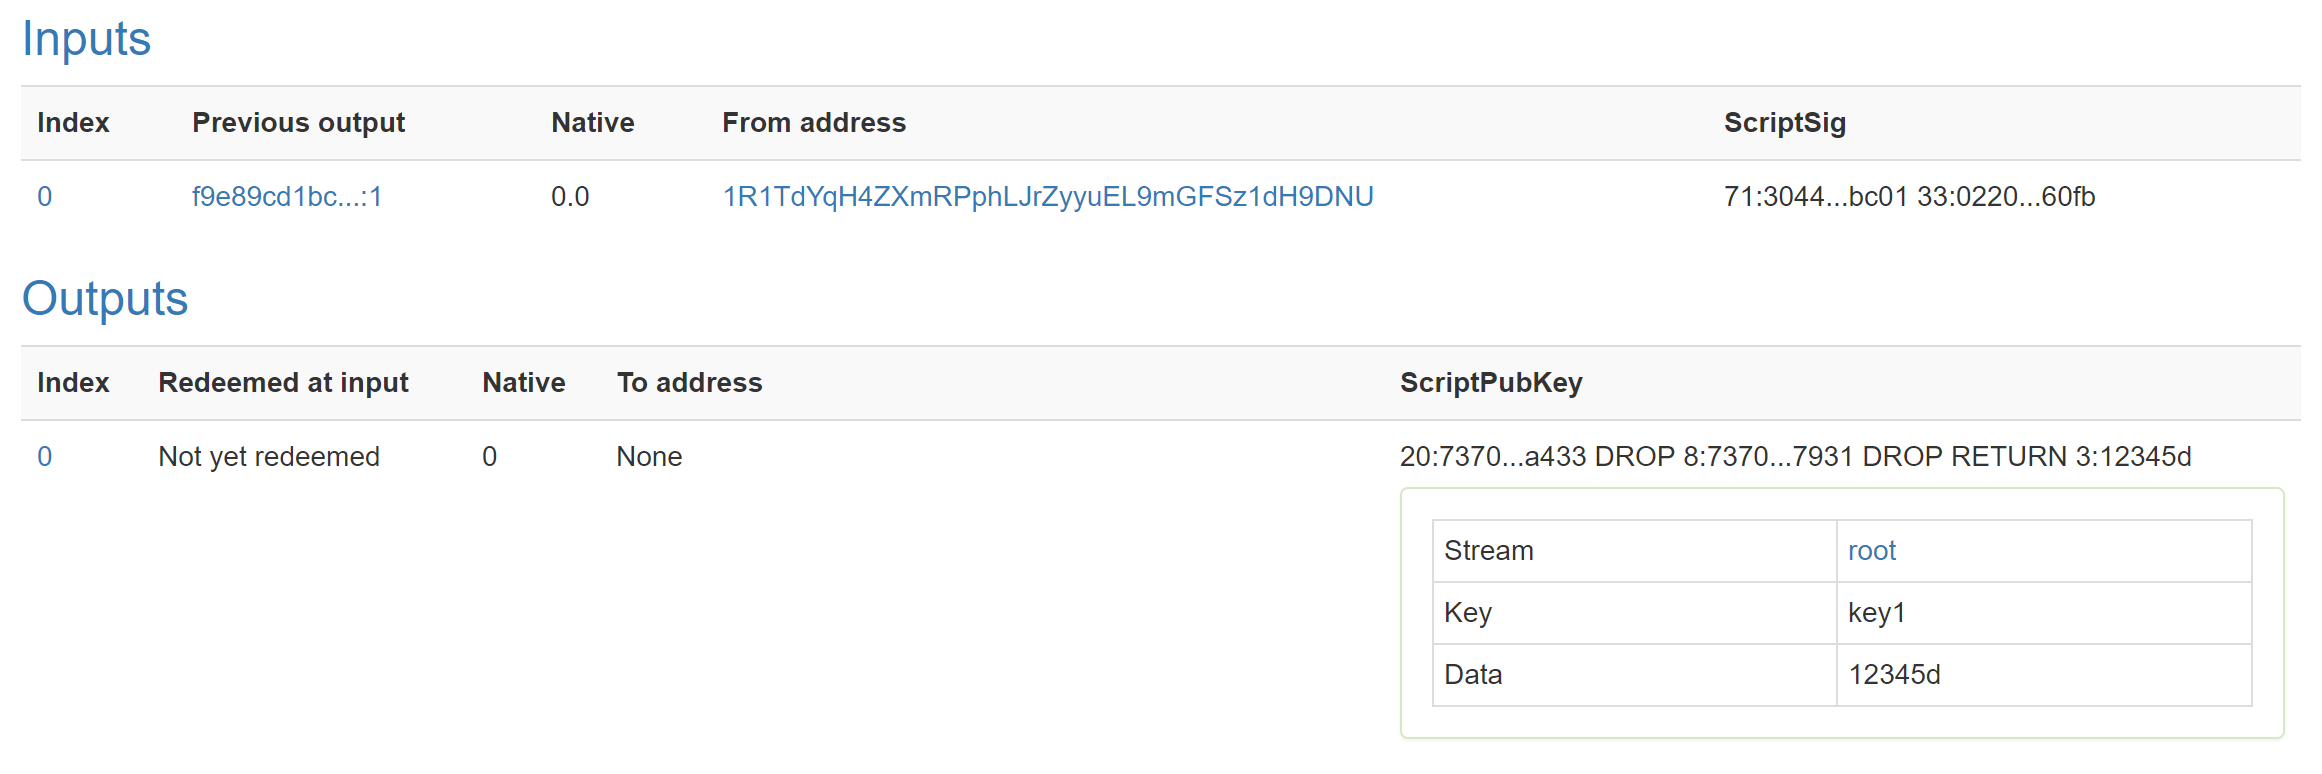
\includegraphics[width=\textwidth]{12.png}
	\caption{Transaktion im Explorer, die Daten enthält}
	\label{fig:12}
\end{figure}

Transaktionen die Daten enthalten, werden von einem Knoten (From address) in einen Stream geschrieben und an niemanden (To address) gesendet. Die Währung der Transaktion ist entsprechend 0. Beim Output der Transaktion wird allerdings eine Tabelle dargestellt, die die versendeten Daten im Feld „Data“, den Key, dem die Daten zugeordnet wurden, und den Stream, in den die Daten geschrieben wurden, enthält. Durch diese Art der Speicherung der Daten durch eine Transaktion und somit den Eingang dieser in die Merkle Root und entsprechend den Hash des validierten Blockes sind auch diese Daten kaum manipulierbar, sofern nicht alle folgenden Blöcke neu berechnet werden.
% !TEX root = ../document.tex
\section{Kritische Reflexion}
\label{sec:Kritik}
% !TEX root = ../document.tex
\section{Fazit}
\label{sec:Fazit}
Zusammenfassend lässt sich sagen, dass Blockchain als Datenbank für eine persistente, manipulationsfreie Datenspeicherung sinnvoll ist. Mit der Software Multichain besteht die Möglichkeit mit wenigen Schritten eine funktionierende Blockchain aufzusetzen.

Das Interesse an einer produktiven Nutzung im unternehmerischen Umfeld wird weiter ansteigen. Der Aspekt der Integrität ist hierfür ausschlaggebend. Im Bereich der Blockchain als Datenbank stehen aber noch viele Fragen aus. Beispielsweise besteht theoretisch die Möglichkeit bei einer Kontrolle von mehr als 50 Prozent der Nodes, die Blockchain zu manipulieren. Des Weiteren spielen auch datenschutzrechtliche Fragen eine Rolle. Beispielsweise lassen sich Blockchains nicht rückwirkend verändern, demnach können keine sensitiven oder illegalen Daten gelöscht werden. In Zukunft müssen weitere Studien über die produktiven Ansätze der Blockchain-Technologie durchgeführt werden.

	
	\clearpage
	\renewcommand{\refname}{Literaturverzeichnis}
	\bibliographystyle{plainnat}
	\bibliography{bibliography}
	% !TEX root = document.tex

\section*{Eidesstattliche Erklärung}
\addcontentsline{toc}{section}{Eidesstattliche Erklärung}

Ich erkläre an Eides statt, dass ich meine Hausarbeit \\ \\
\titel \\ \\
selbstständig und ohne fremde Hilfe angefertigt habe und dass ich alle von anderen Autoren wörtlich übernommenen Stellen wie auch die sich an die Gedankengänge anderer Autoren eng anlehnenden Ausführungen meiner Arbeit besonders gekennzeichnet und die Quellen zitiert habe.
\\ \\

\begin{tabular}{ p{6cm} p{3cm} p{6cm} }
	& & \\\cline{1-1}\cline{3-3}
	\makebox[6cm]{Ort, Datum} & \makebox[3cm]{} & \makebox[6cm]{Unterschrift}
\end{tabular}
	
	\clearpage
	\appendix
	\pagenumbering{roman}
	% !TEX root = document.tex

% iwas.

	
\end{document}
